\documentclass[12pt]{article}

 % Add this line to your preamble
% Language setting
% Replace `English' with e.g. `Spanish' to change the document language
\usepackage[english]{babel}

% Set page size and margins
% Replace `letterpaper' with `a4paper' for UK/EU standard size

\usepackage[top=3cm,bottom=3cm,left=3cm,right=3cm,marginparwidth=1.75cm]{geometry}
	
% Load the setspace package
\usepackage{setspace}
\usepackage{amsmath}
\usepackage{listings}
\usepackage{xcolor}
\usepackage{multirow}
\usepackage{amssymb}
\usepackage{pgfplots}
\usepackage{float}
\usepgfplotslibrary{fillbetween}
\usetikzlibrary{arrows.meta, bending}
\pgfplotsset{compat=newest}
\usetikzlibrary{decorations.markings}
\lstdefinestyle{mystyle}{
    commentstyle=\color{gray},
    keywordstyle=\color{blue},
    numberstyle=\tiny\color{gray},
    stringstyle=\color{purple},
    basicstyle=\ttfamily\footnotesize,
    breakatwhitespace=false,         
    breaklines=true,                 
    captionpos=b,                    
    keepspaces=true,                 
    numbers=left,                    
    numbersep=5pt,                  
    showspaces=false,                
    showstringspaces=false,
    showtabs=false,                  
    tabsize=2
}

\lstset{style=mystyle}

% Useful packages
\usepackage{amsmath}
\usepackage{graphicx}
\usepackage[colorlinks=true, allcolors=blue]{hyperref}
\usepackage{tikz}
\usepackage{natbib}
\pgfplotsset{width=12cm,compat=1.9}
\doublespacing

\bibliographystyle{unsrtnat}

\usetikzlibrary{shapes.arrows, positioning, arrows.meta}


\title{Theoretical framework}
\author{Riccardo Dal Cero}

\begin{document}

\maketitle

\begin{abstract}
    The main idea is to study how and whether the asymmetry of information have an impact on the cleansing effect of
    recession, replicating the model in computer  simulation.
\end{abstract}

\section{Introduction} 


In macroeconomic theory, the investigation of business cycles and long-term growth trajectories traditionally unfolds in
distinct academic silos, drawing a parallel to the distinct realms of quantum mechanics and Einstein's theory of
relativity in physics. This academic segregation, however, obscures a fundamental and profound question: How do business
cycles influence long-term economic growth? The exploration of this question is more than an academic exercise; it
underpins the practical understanding of short-term economic policies, such as automatic stabilizers, and their profound
long-term impacts on the economy. 

Embarking on this exploration, my research primarily dwells in the realm of theory, supplemented by rigorous simulation
and calibration exercises. The intricate complexity of business cycles, particularly evident during periods of economic
downturn and recovery, challenges empirical approaches due to the plethora of confounding variables. Thus, a theoretical
lens, rather than a purely empirical one, is employed to dissect and understand these phenomena. 

Central to this theoretical framework is an examination of the role of financial market frictions during economic
recessions. A key inquiry here is the investigation of policy interventions, such as demand stabilizers, and their
potential effect in attenuating the 'cleansing effect' of recessions. This exploration is pivotal in understanding
whether such policies might inadvertently lead to a reduced economic baseline or steady state in the long term. 
 
The conceptual foundation of this investigation is inspired by an ecological analogy the cyclical dynamics observed
between predator and prey populations in nature. This natural cycle, when observed over extended periods, reveals not
just self-contained oscillations but also underlying trends of population growth for both predators and prey. This
observation leads to a compelling analogy for economic cycles: while they appear as short-term fluctuations, they might
be underpinned by long-term growth trajectories. 

In natural ecosystems, interventions aimed at stabilizing these cycles  such as protecting prey during times of
increased predation  might seem beneficial in the short term. However, such interventions often neglect the critical and
natural process of selection. This interference disrupts evolutionary mechanisms, potentially leading to unforeseen
consequences over time, such as the propagation of traits detrimental to the species' survival and adaptability in
changing environments. 

My thesis extends this analogy to the economic sphere, positing a similar selective mechanism at play in economic
systems. The primary focus is on the recession's cleansing effect, which might be analogous to natural selection in
ecology. This effect could potentially 'weed out' less productive firms, leaving a market landscape dominated by more
efficient players. The exploration aims to decipher whether such an economic 'natural selection' mechanism exists and,
if so, how it shapes the fabric of productivity, innovation, and growth in the long term. Through this lens, the
research endeavors to contribute a nuanced understanding of the intricate interplay between short-term economic
fluctuations and long-term economic evolution, offering insights into the design and implications of economic policies. 
In the following sections, we will delve deeper into specific theories that bridge the gap between business cycles and
long-term economic growth. However, it is beneficial first to embark on a brief historical journey through the evolution
of thought regarding business cycles, to understand the context and development of these interconnected economic
theories. This exploration will provide a foundation for appreciating the diversity of perspectives and the progression
of ideas that have shaped our understanding of the intricate relationship between short-term economic fluctuations and
long-term growth trajectories. 

\section{Business cycle history}
\subsection{Hayek Schumpeter Keynes}
The exploration of business cycle theories represents a cornerstone in the history of economic thought. A prominent
exponent in this realm was Friedrich Hayek, who articulated the complexities of business cycles in relation to economic
equilibrium theory. Hayek's perspective is encapsulated in his own words: 

\begin{quote}
    "The incorporation of cyclical phenomena into the system of economic equilibrium theory, with which they are in
    apparent contradiction remains the crucial problem of Trade Cycle theory; 
    By 'equilibrium theory' we primarily understand the modern theory of the general interdependence of all economic
    quantities, which has been perfectly expressed by the Lausanne School of theoretical economics." \cite{Hay33} 
\end{quote}


In the turbulent era of the early 1930s, the exploration of business cycles was prominently shaped by the contrasting
viewpoints of Friedrich Hayek and John Maynard Keynes, two of the twentieth century's most influential economists.
Hayek's examination of business cycles, as delineated in his seminal work "Monetary Theory and the Trade Cycle,"
\cite{Hay33}, and further elaborated in "The Pure Theory of Capital" \cite{Ha41}, provides a profound analysis
through the lens of monetary theory and its ramifications on capital structure. Hayek posited that economic distortions,
notably those stemming from the artificial depression of interest rates by central banks, precipitate malinvestments
during periods of economic expansion. These malinvestments, especially prevalent in capital-intensive sectors, were
deemed unsustainable, leading inevitably to economic downturns characterized by the correction of these misallocations. 

Conversely, Keynes, in his "The General Theory of Employment, Interest, and Money" \cite{Key36},
approached the business cycle issue from an equilibrium perspective, focusing on the role of aggregate demand in
determining overall economic activity levels. Keynes argued that a shortfall in aggregate demand could lead to
protracted periods of high unemployment, advocating for active government intervention to stimulate demand and
re-establish economic equilibrium. 

Hayek's theoretical framework underscores the intricate relationship between capital investment and monetary
disequilibrium within the business cycle. He elucidates this connection through the concept of inter-temporal
preferences, which dictate the pace of capital investment and the extent of capital accumulation. The decision-making
process regarding the allocation of resources between present dividends and future investment is critical to
understanding the cyclical nature of the economy. Hayek asserts: 

\[ I_t = f(r_t, r_n) \]
\[ r_t < r_n \rightarrow \text{Malinvestment} \]

where \( I_t \) signifies investment at time \( t \), \( r_t \) represents the market interest rate, and \( r_n \)
denotes the natural rate of interest. A divergence between \( r_t \) and \( r_n \), particularly when \( r_t \) is
artificially maintained below \( r_n \), leads to malinvestments. This discrepancy between the market and natural rates
of interest, exacerbated by the expansion of bank credit, serves as the cornerstone of Hayek's business cycle theory.
Hayek further elaborates on the dynamic and temporal aspects of production and investment in "The Pure Theory of
Capital" \cite{Ha41}, where he critically assesses the equilibrium-based economic theories and emphasizes the
importance of understanding the temporal structure of capital. 

Hayek's analysis of monetary disequilibrium and its impact on the business cycle is complemented by his insights into
the mechanisms of bank credit creation and its influence on the natural state of equilibrium in the market for loanable
funds. The expansion of bank credit, which decouples the market rate of interest from the natural rate, instigates
cycles of over-investment and mal-investment, ultimately culminating in inter-temporal economic instability. 

These theoretical perspectives offered by Hayek provide a nuanced understanding of the complexities inherent in the
business cycle, challenging the Keynesian emphasis on aggregate demand and fiscal policy interventions. Hayek's
contributions, particularly in "The Pure Theory of Capital," highlight the significance of capital theory in analyzing
monetary disequilibria and underscore the dynamic and inter-temporal nature of economic activities. 

Thus, while Keynes emphasized stabilizing aggregate demand to achieve equilibrium and mitigate business cycles, Hayek
focused on the inherent dynamism and complexity of economic systems, criticizing equilibrium models for their
oversimplification of the intricate processes that drive economic activities. This divergence in views marked a
fundamental debate in economic theory, shaping the discourse on how economies respond to and recover from periods of
economic downturns. 
\par
\vspace{2cm}
Joseph Schumpeter, another influential economist of the early 20th century, brought a unique perspective to the
discussion of business cycles, one that diverged significantly from both Hayek and Keynes. Schumpeter's approach,
primarily outlined in his theory of "creative destruction," emphasized the role of innovation and entrepreneurial spirit
in economic development and business cycles.  

Schumpeter viewed business cycles as inherent and vital to capitalist economies, driven by the process of innovation.
According to Schumpeter, the entrepreneur is the agent of change, introducing new technologies, products, and methods,
which disrupt existing market equilibria. This process of innovation leads to the destruction of outdated industries and
economic structures, paving the way for new ones. In Schumpeter's framework, the cyclical nature of the economy was a
reflection of this ongoing process of creative destruction, where periods of economic downturns were seen not just as
phases of correction, as Hayek might argue, or as failures of demand, as per Keynes, but as essential for clearing away
the old to make way for the new. 

While Hayek focused on the distortions in capital structure caused by monetary interventions and Keynes emphasized the
role of aggregate demand and government intervention in stabilizing the economy, Schumpeter's perspective highlighted
the evolutionary nature of capitalist economies. He argued that economic fluctuations were natural and necessary, a
process through which economies evolve and adapt over time. Schumpeter's theory thus provided a more dynamic view of
capitalism, recognizing the disruptive yet progressive role of innovation and entrepreneurship in shaping economic
landscapes. 

Schumpeter's contribution added a dimension of evolutionary change to the understanding of business cycles,
contrasting with Hayek's emphasis on monetary theory and capital structure, and Keynes's focus on equilibrium and
aggregate demand. Schumpeter's insights into the transformative power of innovation offered a more optimistic view of
economic downturns, seeing them as opportunities for new growth and advancements, the predecessor of the idea of
cleansing effect. 
 
\subsection{Theories Connecting Business Cycles to Long-Term Growth}

In the domain of economic theory, the relationship between business cycles (BC) and long-term growth is dissected into
two principal schools of thought. The conventional viewpoint suggests that long-term growth is chiefly propelled by
technological progress. Within this framework, technological advancements are often viewed as exogenous—arising outside
the economic model's explanatory scope, as highlighted in the seminal contributions of \cite{Sol56} and \cite{Swa56}.
This perspective treats technological progress as an independent variable that exerts influence on economic growth
without being influenced by the economy's internal dynamics. 

Contrastingly, an alternative strand of theoretical work aims to endogenize technological progress, weaving it into the
fabric of the economic process. These models embed factors such as incentives for innovation, the value of education,
and the accumulation of knowledge through economic activities, epitomizing the 'learning by doing' paradigm. A prominent
example of this approach is found in \cite{Sta90}, which posits technological progress as an emergent property of
economic behavior and incentives, rather than a mysterious external force. 

A critical aspect of the 'learning by doing' model is its premise that technological frontiers are contingent upon the
existing knowledge base, which expands primarily through practical experience. Consequently, periods of economic
expansion witness a sharp increase in the knowledge stock, driven by higher employment levels, whereas recessions tend
to stabilize or even diminish this stock due to reduced employment rates. This dynamic suggests that economies devoid of
cyclical fluctuations might attain superior steady-state growth, as employment remains consistently high, fostering
continuous technological advancement. From this perspective, the concept of a 'cleansing effect'—whereby economic
downturns eliminate low-productivity jobs and ostensibly strengthen the economy—is challenged. The elimination of even
low-productivity roles can erode the overall knowledge base. 

Such theories reframe the discourse on stabilization policies, particularly fiscal interventions, by highlighting their
role in sustaining employment and, by extension, supporting the technological frontier even in downturns. 

To illustrate this theory's implications more vividly, consider a nuanced example: an antiquated factory with limited
land resources discovers an innovative method to utilize an old tractor more efficiently. Despite the ingenuity of this
breakthrough, if the broader economy has moved beyond the technology that the tractor represents, the innovation might
not significantly contribute to the overall knowledge stock or push the technological frontier forward. This scenario
prompts a fundamental inquiry: does innovation at the lower end of the skill spectrum or within outdated technological
contexts meaningfully advance the technological frontier? Or, would it be more beneficial for economic growth to
transition such small-scale innovations into larger entities equipped with modern technologies? 

One significant critique concerns the disparity in learning opportunities across different sectors and among
individuals. The model's premise of uniform learning opportunities does not always align with the reality that some
industries, such as the technology sector, offer rapid innovation and learning environments compared to more traditional
manufacturing industries, where the pace of learning and innovation may be inherently slower due to the nature of the
work processes involved.

Furthermore, the model may not adequately address the issue of structural unemployment that can arise from technological
advancements. As certain workers benefit from "learning by doing," leading to increased productivity, others may find
their skills becoming obsolete due to automation and other technological changes. This dynamic is evident in the
automation of routine manufacturing jobs, which, while fostering "learning by doing" in fields like robotics and
software engineering, simultaneously leads to structural unemployment for workers displaced by these technologies.

Another point of contention is the potential for diminishing returns to learning. The assumption that "learning by
doing" continuously fuels growth may not hold up against the reality that initial rapid gains in productivity tend to
taper off as workers gain proficiency, suggesting that the benefits of learning may diminish over time.

The model also potentially overlooks the externalities and spillover effects associated with "learning by doing."
Technological advancements in one firm or sector do not automatically translate into broader economic growth if these
advancements remain isolated and do not benefit other sectors or industries. This is illustrated by a software company
that develops cutting-edge algorithms, enhancing its productivity but failing to contribute to the wider economy if the
knowledge remains proprietary.


This nuanced exploration challenges the simplistic notion of 'learning by doing' by questioning the value and impact of
incremental innovations within the broader economic and technological ecosystem. It underscores the complexity of
technological progress and its interplay with economic dynamics, inviting a deeper investigation into the mechanisms
that drive long-term growth and the role of policy in nurturing an environment conducive to continuous innovation and
knowledge expansion. 

The contemporary perspective on technological advancement, when viewed as a product of incremental contributions from
every market participant, appears overly simplistic. A more accurate depiction of technological progress recognizes it
as predominantly driven by those at the forefront of research. The expansion of the technology frontier is essentially
shaped by the knowledge and breakthroughs of these leading-edge innovators. Other entities in the economy adopt these
innovations at varying paces, influenced by the associated adoption costs. While firms that are not at the innovation
frontier may achieve marginal efficiency gains through adoption, the impact of such improvements is often minimal. These
marginal innovations are frequently a reflection of the adopting firms' constraints, particularly their inability to
invest in more advanced and expensive technologies. Consequently, these incremental innovations have limited potential
for widespread diffusion, as they stem from a position of necessity rather than pioneering advancement. 

Another theory describe a recession as a period in which the opportunity cost of investing in a productivity enhancing
projects is lower since the workforce is not fully in demand to produce goods. Doing this would lead in theory to higher
productivity in the period of expansion. The key role here is that the productivity-enhancing activity is costly and thus
divert capital and labor force from production as Hayek \cite{Hay33} explained. 
For this view to be valid two key aspects should be true at the same time: in the first place the
expectations about the length of the recession should reinter in the short-term otherwise it is cheaper to destroy some
production units (labor and capital) to accommodate the slow in demand. The last condition is that internal resources
must be less costly than external ones, however, it would be cheaper to higher more skilled workers and fire the low-skill
one. An additional remark is the this theory describes all those initiatives like worker formation that affect only
marginally the productivity of a firm. It misses the main mechanics in which a firm can increase its productivity sharply: thorough technical
innovation, and to do so you need a research program where the workforce is fully dedicated to it and not
diverted from production.

Another theory posits that recessions offer a period in which the opportunity cost of investing in
productivity-enhancing projects are lower, primarily because the workforce is not fully engaged in producing goods.
Theoretically, this would lead to higher productivity during subsequent periods of expansion. A crucial element in this
perspective is the acknowledgment that productivity-enhancing activities are expensive, thereby diverting capital and
labor away from immediate production, a concept Hayek \cite{Hay33} elucidated. 

For this viewpoint to hold, two critical conditions must be concurrently satisfied: firstly, expectations regarding the
duration of the recession must be short-term. If the recession is anticipated to be prolonged, it becomes economically
viable to dismantle some production units (both labor and capital) to adjust to reduced demand. Secondly, the cost of
utilizing internal resources for such productivity-enhancing ventures must be lower than the cost of acquiring external
resources. Otherwise, it might be more economical to hire more skilled workers and lay off less skilled ones.  

An additional observation about this theory is that it accounts for initiatives like worker training, which only
marginally affect a firm's productivity. This overlooks the primary mechanism through which a firm can significantly
boost its productivity: through technical innovation. To achieve substantial innovation, a dedicated research program is
essential, where the workforce is fully committed to innovation efforts rather than being diverted to current production
tasks. This highlights a gap in the theory, suggesting that while reallocating resources during recessions may offer
some productivity benefits, the most dramatic productivity improvements are likely achieved through focused
innovation and research activities, not merely through the opportunistic reallocation of resources during economic
downturns. 

An intricate theory that elaborates on the dynamics of economic recessions and the associated lower opportunity costs is
grounded in the concept of labor hoarding, as discussed in the seminal work by Clark \cite{Cla73}. This theory posits
that firms maintain employment levels higher than what immediate efficiency metrics might dictate. The rationale behind
such a strategy is to prepare for a potential surge in demand, ensuring that the firm can quickly ramp up production
without the delays associated with recruiting and training new employees. However, this strategic maneuver towards the
internal possibility frontier—where firms optimize their readiness for future demand—does not manifest as observable
changes in employment rates. Consequently, this leads to discrepancies or residuals in the statistical series of
employment, which do not align with what might be considered the level of optimal employment, a phenomenon further
analyzed in the work of \cite{BurnCrai93}. 

This labor hoarding theory offers a partial explanation for the strong pro-cyclically of measured productivity. During
economic upturns, firms can immediately respond to increased demand using their hoarded labor, thereby appearing more
productive. Conversely, during downturns, the reluctance to shed this excess labor, due to the anticipation of future
demand recovery, results in lower observable productivity levels. This behavior underscores a strategic depth in firm
management, navigating through the cyclical economic waves by balancing between immediate efficiency and long-term
responsiveness. 

Expanding on this foundation, it becomes evident that the decision to engage in productivity-enhancing activities during
recessions is not merely a reaction to lower opportunity costs but also a strategic consideration influenced by
expectations of the recession's duration and the comparative costs of internal versus external resources. If firms
anticipate a short-lived recession, the logic of hoarding labor and investing in internal productivity initiatives
becomes compelling. However, this strategy hinges on the assumption that improving the skill set of the existing
workforce or reallocating resources towards innovation is less costly than the alternative—acquiring new, possibly more
skilled labor post-recession. 

The opportunity cost (OC) approach closely aligns with the theory of labor hoarding, which seeks to elucidate the
pronounced procyclicality of measured productivity. This observation implies that during economic downturns, firms
appear to retreat towards the interior of their production possibility frontier, opting for a strategic reduction in
operational efficiency rather than workforce downsizing. This strategy is partly attributed to the invisible nature of
one crucial input—effort—to statisticians, and the economic rationale that, given the costs associated with employee
turnover, it proves more economically viable for firms to dial back effort during slumps instead of terminating
employment. 

An intriguing alternative to diminishing effort is the redirection of employee tasks from immediate production roles to
undertakings that bolster the firm's long-term productivity. At first glance, this strategy bears a resemblance to labor
hoarding but carries the added outcome that these so-called shadow activities, embraced during recessions, eventually
manifest as enhancements in total factor productivity. 

The concept of adjustment costs does not singularly confine firms from adapting their production factors according to
operational necessities. This opportunity cost mechanism could theoretically extend to a macroeconomic scale,
influencing individual entities via price adjustments. During periods marked by diminished production value, the
immediate returns from production activities (e.g., wages for workers) decline in comparison to alternative endeavors,
notably human capital accumulation, whose benefits are pegged to future earnings. This economic mechanism could
precipitate a resource reallocation towards these alternative activities. The empirical observation that education
durations tend to extend during economic recessions lends credence to this argument. Nevertheless, with the exception of
leisure, most sectors shadow the movements of aggregate GDP. Thus, if productivity-enhancing activities (PEAs) are to
occur during recessions, the resource reallocation process must predominantly unfold within the firms themselves. 

One notable deviation might be labor reallocation. As demonstrated by \cite{DavHalt92}, job destruction exhibits a
more countercyclical pattern compared to job creation. Viewing job reallocation through the lens of both destruction and
creation suggests a countercyclical trend, positing job reallocation as an investment in cultivating superior
firm-worker matches, thereby sowing the seeds for heightened productivity in the future. \cite{DavHalt92}further
postulate, within the framework of a model featuring a representative agent, that economic recessions present an optimal
window for labor reallocation, highlighting a strategic dimension to workforce management during downturns that might
ultimately contribute to long-term productivity gains. 
 
The "lame ducks" theory, initially proposed by \cite{CabHarm94}, offers an intriguing perspective on
recessions as mechanisms that phase out less profitable, outdated capital. This theory delineates how the destruction of
older units during downturns is more pronounced than the construction of new ones, characterizing recessions as periods
marked by the systematic elimination of obsolete capital, hence the moniker "lame ducks" theory. Notably, this framework
sheds light on observations documented by \cite{DavHalt92}, positioning it as a prominent theoretical
approach that will be delved into more thoroughly in subsequent discussions. 

Despite its insights, this model lacks consideration of the financial dimensions of firms, an aspect addressed by the
theoretical work of \cite{OsePap17}. Their research weaves the financial decision-making process into the
broader context of intertemporal capital decisions, highlighting how financial frictions influence the lender's
participation constraint. The study reveals that, despite financial frictions, the cleansing effect of recessions on
productivity persists, potentially leading to a more pronounced productivity surge during expansion phases. This
analysis serves as a pivotal foundation for the new theoretical framework introduced in this thesis, marking a
significant departure from traditional views and emphasizing the multifaceted impact of recessions on firm productivity
and economic recovery. 

In the forthcoming sections, we will delve into the empirical evidence presented by \cite{DavHalt92} in their
seminal works from 1990 and 1992, which lay the groundwork for our discussion. Following this, we will explore the
theoretical underpinnings that form the basis of the new, streamlined theoretical framework introduced in this thesis.
Our examination begins with the insights of \cite{CabHarm94}, focusing on the interplay between the
destruction and creation margins in economic cycles. Subsequently, we will delve into the work of \cite{OsePap17}
(2017), which sheds light on the financial dimensions, particularly how capital lending frictions can precipitate
misallocations. These studies collectively inform the development of our theoretical framework, setting the stage for a
comprehensive analysis of economic dynamics and firm behavior during recessions. 
\section{Literature review of empirical studies}
\subsection{Emprical findings}
This analysis juxtaposes two pivotal studies that dissect business cycle dynamics through the lens of labor market
fluctuations and job reallocation. The first, by \cite{DavHalt92}, scrutinizes job reallocation during
recessions, employing data from the U.S. manufacturing sector. The second study, by \cite{BlaDia90},
concentrates on labor flows throughout business cycles. Both studies utilize labor data from the Current Population
Survey (1968-1986) and manufacturing data from the Federal Bureau of Labor Statistics up to 1981, later complemented by
the Longitudinal Research Database. These works collectively illuminate the dynamic interplay of job creation and
destruction, offering a nuanced understanding of labor market volatility and its implications for economic cycles.
Further exploration will include an analysis of Haltiwanger's findings and their application to understanding
the Great Recession's impact on the labor market in his paper \cite{FosHal16}
\paragraph{Reallocation cleansing or not?}
This study meticulously investigates the variance in employment changes at the establishment level within the U.S.
manufacturing sector from 1972 to 1986, focusing on the gross creation and destruction of jobs and the rate of job
reallocation across plants. Leveraging an extensive dataset from the Annual Survey of Manufactures, it provides a
detailed examination of how job and worker reallocation contribute to understanding employment dynamics and the cyclical
nature of the labor market. The findings reveal significant rates of job turnover within specific industry sectors and
elucidate the relationship between job reallocation and various plant characteristics such as age, size, and ownership
type. Moreover, the research discusses the persistence and concentration of job creation and destruction, highlighting
their implications for long-term employment trends and worker mobility. Through analyzing the interplay between
establishment-level job flows and broader labor market states, this paper contributes valuable insights into the
mechanisms of labor reallocation and the structural factors driving employment heterogeneity in the manufacturing
sector. 

The key concept behind the \cite{DAvHalt90,DavHalt92} studies is that the measure of reallocation is given by the sum of job
or capital creation and destruction. In the first place lets get some definitions that are used in the paper:
The analysis in this paper establishes a straightforward link between the gross job flow metrics and the size-weighted
distribution of establishment growth rates. Gross job creation is determined by aggregating employment increases in both
growing and newly established firms within a sector. In a similar vein, gross job destruction is assessed by totaling
employment declines in contracting and ceasing operations. This methodological approach allows for a comprehensive
evaluation of employment dynamics, highlighting the pivotal role of establishment size and growth in understanding
sectoral labor market fluctuations. 
To measure Total Factor Productivity (TFP) at the establishment level, they construct an index following the methodology
similar to \cite{baily1992productivity} and subsequent studies. The formula for the index is:  

\[ \ln(\text{TFP}_{et}) = \ln(Q_{et}) - a_K\ln(K_{et}) - a_L\ln(L_{et}) - a_M\ln(M_{et}) \]

In this equation, \(Q\) represents real output, \(K\) stands for real capital, \(L\) denotes labor input, and \(M\)
signifies real materials used, with \(a\) representing the factor elasticities. The subscript \(e\) refers to individual
establishments, while \(t\) denotes time, allowing for a dynamic analysis of productivity changes across establishments. 
The methodology for measuring Total Factor Productivity (TFP) at the establishment level involves detailed component
measurements. Nominal output is calculated by summing total shipments with inventory
changes, adjusted by industry-specific deflators from the NBER-CES Manufacturing Industry Database. Capital is
quantified using the perpetual inventory method for structures and equipment, while labor input comprises total hours
worked by both production and nonproduction workers. Materials, including physical materials and energy, are measured
and deflated by industry-specific indices, with all values expressed in 1997 constant dollars. Factor elasticities are
determined using industry-level cost shares, with adjustments made to account for industry differences in TFP
calculations, ensuring comparisons control for sectoral disparities. 
The first question they try to address is Did Reallocation Dynamics Change in the great recession?
\begin{figure}
    \centering
    \includegraphics[scale = 0.6]{Plot1.1.png}
    \caption{Figure Job flows and the business cycle. Authors' calculations using Business
    Dynamics Statistics (annual), Business Employment Dynamics (quarterly), and
    the Current Population Survey. Cycle is the change in the unemployment rate.
    }
    \label{plot:1.1}
\end{figure}
The graph also depicts the fluctuations in the unemployment rate, clearly demonstrating that periods of rising
unemployment are typically marked by increased job losses and decreased job creation. However, the trend took a notable
turn during the Great Recession. Specifically, while job losses did surge in the 2008-2009 period, the most remarkable
change was the significant drop in job creation beginning in 2007 and extending through 2010. Additionally, there is an
observable long-term decline in job flow dynamics, a topic for further discussion. 

To corroborate these findings and delve into more granular data, they utilized the Business Employment Dynamics (BED)
statistics for the U.S. private sector. The BED's quarterly data from the second quarter of 1990 to the first quarter of
2012 (Panel B of the figure) underscores the annual trends, showing that recessions typically involve higher job
destruction and lower job creation rates. The period starting in 2007 stands out for a particularly steep decline in job
creation, a trend that is more pronounced in the BED data. The BED series also highlights that the sluggish recovery
from the Great Recession up to early 2012 is primarily attributable to weak job creation rather than enduringly high job
destruction rates. This pattern, confirmed by other datasets such as the Job Openings and Labor Turnover Survey (JOLTS),
persisted beyond the first quarter of 2012. 

Adding to this, job creation during the Great Recession was as low as it has been at any time in the past 30 years, as
illustrated in the figure. Moreover, job reallocation (the sum of job creation and destruction) reached its lowest point
in 30 years during the Great Recession and its immediate aftermath. When comparing the Great Recession to the early
1980s recession, the rate of job reallocation was 28* in 2009, in stark contrast to 35* in 1983 (both periods represent
peaks in job destruction and are measured using March-to-March Business Dynamics Statistics data). These patterns are
partly driven by significant downward trends in job flows, as evidenced in both the Business Dynamics Statistics (BDS)
and the BED data. Although exploring the causes of these declining trends in job flows is beyond the scope of this
analysis, it is clear that these trends are significant and have been taken into account in the analysis. 

Moreover, the authors show how the patterns change considerably in the great recession, particularly regarding how the
creation and destruction rate of jobs respond to the sharp fall in demand. They found as expected from \cite{CabHarm94}
that the creation rate of new jobs slower before the crisis spreads out and than the destruction rate increases when it is
not possible to fully accommodate the decrease in demand only stopping new labour hiring. They asses that during the
Great Recession this pattern changes in particular the fraction of net employment contraction accounted by a job
reduction is higher than 0.5, while for all the previous recessions it was way below 0.4 as shown in the table.
\begin{table}[H]
    \centering
    \caption{
    Share of Change in Net Employment Growth Due to Change in Job Creation in Periods of Net Contraction}

    \begin{tabular}{lccc}
    \hline & \multicolumn{2}{c}{ National } & State \\
    \cline { 2 - 3 } Period & BDS (Annual) & BED (Quarterly) & BDS (Annual) \\
    \hline Pre-Great Recession & .21 & .28 & .39 \\
    Post-2007 & .61 & .59 & .65 \\
    \hline
    \end{tabular}
    \label{tab:1.2}
\end{table}

This analysis is based on the authors' computations using data from the Business Dynamics Statistics (BDS) and Business
Employment Dynamics (BED). The methodology hinges on the principle that net employment change equals job creation minus
job destruction. For any period(s) of net employment decrease lasting at least one period, both the total change in net
employment growth and the total change in job creation are aggregated over the full duration of consecutive net
contraction periods. Furthermore, these aggregated changes are then further combined within the periods outlined in the
analysis. The proportion mentioned refers to the fraction of the total aggregated change in net employment growth during
the specified timeframe that is attributed to the total change in job creation within the same timeframe. Specifically,
the BDS data spans from 1981 to 2007 for the pre-Great Recession era and from 2008 to 2011 for the post-2007 era. For
the BED, the pre-Great Recession period covers from the second quarter of 1990 to the third quarter of 2007, and the
post-2007 era from the fourth quarter of 2007 to the first quarter of 2012. It's important to note that these
calculations are applied solely to periods experiencing a net decrease in employment growth. For instance, this applies
to the period from the fourth quarter of 2007 to the first quarter of 2010 for the BED data. Regarding the BDS National
Annual data, there are six years of net employment contraction, with two of those years occurring after 2007. In the BED
Quarterly data, there are twenty-two quarters of net contraction, with nine quarters following 2008. For the BDS State
Annual data, there are 393 state-year instances of net contraction, with 112 of those instances occurring after 2007. 

Another way to see this change in patterns is regressing job creation rate, job destruction rate, and Reallocation rate
to Cyle an iteration between a Great Recession dummy and the cycle and a trend. The results are shown in the table 3.
\begin{table}
    \centering
    \caption{Job Flows and Change in the Unemployment Rate at the State-Level (Annual), 1981-2011}
    \begin{tabular}{|c|c|c|c|}
    \hline & \begin{tabular}{l} 
    Job Creation \\
    Rate
    \end{tabular} & \begin{tabular}{c} 
    Job Destruction \\
    Rate
    \end{tabular} & Reallocation Rate \\
    \hline Cycle & \begin{tabular}{l}
    $-.631 ***$ \\
    $(.046)$
    \end{tabular} & \begin{tabular}{l}
    $1.194 ***$ \\
    $(.053)$
    \end{tabular} & \begin{tabular}{l}
    $.563 ***$ \\
    $(.068)$
    \end{tabular} \\
    \hline GR $\times$ cycle & \begin{tabular}{l}
    $-.371 ***$ \\
    $(.079)$
    \end{tabular} & \begin{tabular}{l}
    $-.421^***$ \\
    $(.079)$
    \end{tabular} & \begin{tabular}{l}
    $-.793 ***$ \\
    $(.128)$
    \end{tabular} \\
    \hline Trend & \begin{tabular}{l}
    $-.168***$ \\
    $(.010)$
    \end{tabular} & \begin{tabular}{l}
    $-.136 ***$ \\
    $(.011)$
    \end{tabular} & \begin{tabular}{l}
    $-.304***$ \\
    $(.020)$
    \end{tabular} \\
    \hline
    \end{tabular}
    \footnote{$-N=1,581$. GR is a dummy variable equal to one for years from 2008 to 2010 (job flows from March 2007 to March 2010). The cycle is the state-year change in the unemployment rate. All specifications include state fixed effects. Standard errors in parentheses are clustered at the state level.
    $$
     because * \quad p<.01 \text {. }
    $$}
    \label{tab:1.2}
\end{table}
The authors delve into the nuances of state-level job flow dynamics by leveraging the variation in the relationship
between cyclical economic indicators and job flows across different states. Their methodological approach is rooted in
conducting descriptive regressions that not only link job flows to a selected cyclical indicator but also incorporate an
interaction term that captures the distinctive economic conditions of the Great Recession period alongside the cyclical
variable. To achieve this, they meticulously utilize changes in the unemployment rate at the state level as a proxy for
economic cycles. Recognizing the persistent negative trend in job flows across the board, the authors judiciously
incorporate a linear trend into their regression models to adequately account for this overarching pattern. 

The findings from these regressions are illuminating, revealing that cyclical fluctuations predominantly explain a
substantial portion of the variance observed in job flows, particularly with respect to the job destruction rate. This
observation is in line with the theoretical framework posited by \cite{CabHarm94}, which suggests that the
margin of job destruction exhibits a higher sensitivity to cyclical downturns compared to the job creation margin. A
striking aspect of their analysis is the significant and negative interaction observed between the cyclical variable and
the Great Recession dummy variable, indicating that this period was characterized by a pronounced decrease in the rate
of new job openings, whereas the rate of job layoffs was not as severely affected as it had been in other recessions.
This pattern underscores the profound and distinctive impact of the Great Recession, which led to a dramatic downturn in
job creation, surpassing the declines observed in job destruction rates and deviating markedly from the trends seen in
prior economic downturns. 

Furthermore, the analysis sheds light on the behavior of the job reallocation rate during the Great Recession, which, in
a departure from its traditionally pro-cyclical nature observed in earlier recessions, switched signs, indicating a
contraction in job reallocation. This reversal is particularly noteworthy as it signifies a shift towards less job
reallocation, thereby challenging the conventional understanding of job flow dynamics during economic downturns. 

An important contribution to this discourse comes from studies that emphasize the significant role of young businesses
in the observed decline in job creation rates, particularly highlighted in the research by \cite{fort2013firms}. These young
businesses, defined as entities with less than five years of operation, exhibit a markedly higher responsiveness in
their job creation margin, especially in the aftermath of the 2007 financial crisis. This responsiveness is contrasted
with the behavior of older firms, which, although also experiencing shifts in their job creation and destruction
margins, do not demonstrate the same level of sensitivity as their younger counterparts. The distinction between young
and old firms becomes even more pronounced when examining the destruction margin, where young firms again show greater
responsiveness, underscoring the differential impact of economic cycles based on firm age. 
\begin{figure}
    \centering
    \includegraphics[scale = 0.54]{Plot1.2.png}
    \caption{Job flows by age, 1981-2011. Authors' calculations on Business Dy-
    namics Statistics. Young is for establishments owned by firms less than 5 years old.
    Mature is for establishments owned by firms 5 or more years old. Job flows are
    establishment-based and are classified by firm age characteristics.
    }
    \label{plot:1.1}
\end{figure} 
The second question that the authors try to address is: Did the Cleansing Effect change during the Great Recession?
To address this question the authors use a regression that examines the relation between the growth and survival
dynamics of the incumbent establishment to productivity. The specification that they imply is the following 
The specification is defined as follows:
\[ Y_{es,t+1} = \lambda_s + \lambda_{t+1} + \beta(\text{TFP}_{es,t}) + \gamma(\text{Cycle}_{s,t+1}) + \delta(\text{TFP}_{es,t} \times \text{Cycle}_{s,t+1}) + X'_{es,t}\mathbf{V} + \epsilon_{es,t+1}; \]
where \(e\) represents the establishment, \(s\) denotes the state, and \(Y\) encompasses a series of outcomes. TFP
refers to the deviations in total factor productivity from the average within each industry by year, and Cycle
represents the variation in the state-specific unemployment rate from time \(t\) to \(t+1\). The model assesses three
distinct outcomes (all calculated from \(t\) to \(t+1\)): "Overall Growth" (combining continuing operations and exits),
"Exit," and "Conditional Growth" (considering only those that continue, i.e., no exiters). 
They used data from 1981-2010 controlling per year and state effects. In order to assess if the Great Recession was
different from previous recessions the added iteration terms with a dummy variable representing the Great Recession. 
The specification became the following:
The refined model is expressed as:
\[ Y_{es,t+1} = \lambda_s + \lambda_{t+1} + \beta(\text{TFP}_{es,t}) + \gamma(\text{Cycle}_{s,t+1}) + \delta(\text{TFP}_{es,t} \times \text{Cycle}_{s,t+1}) + \xi(\text{GR}_{t+1} \times \text{TFP}_{es,t}) + \mu(\text{GR}_{t+1} \times \text{Cycle}_{s,t+1}) + \phi(\text{GR}_{t+1} \times \text{Cycle}_{s,t+1} \times \text{TFP}_{es,t}) + X'_{es,t}\mathbf{V} + \epsilon_{es,t+1}; \]
where GR signifies a dummy variable for the Great Recession, assigned a value of 1 during the years 2007 to 2009. This
the model takes into account the impact of the Great Recession by including interaction terms between the Great Recession
dummy (GR), changes in the state-specific unemployment rate (Cycle), and deviations in total factor productivity (TFP)
from the industry-year averages.
 The results are shown in the following table
 \begin{table}[H]
    \centering
    \caption{Reallocation and Productivity over the Business Cycle}
    \begin{tabular}{|c|c c c c c c|}
    \hline & \multicolumn{2}{c|}{Overall Gr.Rat. (Cont + Exit)} & \multicolumn{2}{c|}{Exit} &
    \multicolumn{2}{c|}{Cond. Gr.Rat.(Cont.)} \\
    & \multirow{2}{*}{prova}\\
    \hline & (1) & (2) & (3) & (4) & (5) & (6) \\
     \multirow{2}{*}{TFP} & $.157^{***}$ & $159^{***}$ & $-.060^{***}$ & $-.060^{**}$ & $.041^{**}$ & $.042^{*}$ \\
    & $(.006)$ & $(.006)$ & $(.003)$ & $(.003)$ & $(.003)$ & $(.003)$ \\
     \multirow{2}{*}{Cycle} & $-3.307^{**}$ & $-2.961^{*}$ & $.671^{*}$ & $.497^{*}$ & $-2.143^{**}$ & $-2.128$ \\
    & $(.459)$ & $(.483)$ & $(.176)$ & $(.179)$ & $(.247)$ & $(.286)$ \\
     \multirow{2}{*}{TFP $\times$ cycle} & $1.542^{***}$ & $2.182^{***}$ & $-.655^{***}$ & $-.927^{**}$ & $.494$ & $.534$ \\
    & $(.643)$ & $(.862)$ & $(.226)$ & $(.265)$ & $(.412)$ & $(.567)$ \\
     \multirow{2}{*}{GR $\times$ TFP} & & $.030$ & & $-.018^{*}$ & & $-.005$ \\
    & & $(.023)$ & & $(.011)$ & & $(.011)$ \\
     \multirow{2}{*}{GR $\times$ cycle} & & $-3.116^{*}$ & & $1.581$ & & $-.126$ \\
    & & $(1.349)$ & & $(.523)$ & & $(.770)$ \\
     \multirow{2}{*}{GR $\times$ TFP $\times$ cycle} & & $-2.961^{*}$ & & $1.466^{***}$ & & $.066$ \\
    & & $(1.619)$ & & $(.684)$ & & $(.764)$ \\
    \hline Year FE & Yes & Yes & Yes & Yes & Yes & Yes \\
     State FE & Yes & Yes & Yes & Yes & Yes & Yes \\
     Firm size class FE & Yes & Yes & Yes & Yes & Yes & Yes \\
     $N$ (millions) & 2.2 & 2.2 & 2.2 & 2.2 & 2.1 & 2.1 \\
    \hline
    \end{tabular}
    \footnote{SOURCE: Authors' calculations based on the Annual Survey of Manufactures, the Census of Manufactures, and the Longitudinal Business Database.}
    \footnote{NOTE: Regressions are weighted using propensity score weights, detailed in the online appendix. Standard errors, in parentheses, are clustered at the state level. Employment growth and exit rates are measured from period $t$ to $t+1$. Exit regression employs a linear probability model, defining exit as 1 if the establishment is active in period $t$ but not in $t+1$. TFP represents the deviation of establishment-level log TFP from its industry-year mean. GR is a dummy variable for the years 2007 to 2009, reflecting the impact of the Great Recession from March 2007 to March 2010. Cycle measures the change in the state-year unemployment rate. Establishment size (log employment) at time $t$ is included as a control.}  
\end{table}
The regression analysis presented in the table offers insightful observations on how the Great Recession exacerbated the
effects on overall growth rates compared to other periods of economic downturns. A critical aspect to highlight is the
interaction between the Great Recession dummy variable (GR) and the cycle, which denotes changes in the state-year
unemployment rate. This interaction is particularly important and statistically significant, with one coefficient
significant at the 5\% level and the other at the 1\% level. This suggests that the economic dynamics during the Great
Recession had a distinct and profound impact on reallocation and productivity across businesses. 

The coefficient for the GR $\times$ cycle interaction being significant implies that the Great Recession intensified the
negative effects of the business cycle on overall growth rates. This finding is notable because it underscores the
unique severity of the Great Recession, distinguishing it from previous economic downturns. Specifically, the negative
coefficient indicates that during the Great Recession, the adverse effects of an economic downturn on job creation and
overall business growth were more pronounced. This could be attributed to a range of factors, including tighter credit
conditions, greater uncertainty, and possibly more significant structural shifts in the economy that affected businesses
more severely during this period. 

Moreover, the presence of significant interaction terms involving TFP (total factor productivity), the cycle, and the
Great Recession dummy highlights the complex relationship between productivity, economic cycles, and major economic
crises. The analysis suggests that the Great Recession not only impacted the rate of job creation and destruction but
also influenced how productivity interacts with the business cycle to affect economic outcomes. 

To have a better comprehension the authors use the regression coefficients to estimate the difference in the outcomes
between an establishment firm with one standard deviation above and below the industry year mean, differing between
older and younger firms the results are depicted in the following plot.
\begin{figure}{ht}
    \centering
    \title{A. Overall Growth(Cont. + Exiters)}
    \includegraphics[scale = 0.35]{Plot1.3.png}
    
    \label{plot:1.3}
\end{figure} 
\begin{figure}{ht}
    \centering
    \title{B.Exit Rates}
    \includegraphics[scale = 0.35]{Plot1.4.png}
    
    \label{plot:1.3}
\end{figure} 
\begin{figure}{ht}
    \centering
    \title{C.Conditional Growth (Continuers only)}
    \includegraphics[scale = 0.35]{Plot1.5.png}
    
    \label{plot:1.3}
    \caption{Differences in growth rates between high-productivity and low-
    productivity establishments, normal times. Authors' calculations on Annual Survey
    of Manufactures, Census of Manufactures, and Longitudinal Business Database.
    Depicted are the predicted difference in growth rates (panels A and C, high minus
    low) and the predicted difference in probability of exit (panel B, low minus high)
    between an establishment one standard deviation above industry-by-year mean
    productivity and an establishment one standard deviation below industry-by-year
    mean productivity. Normal is zero change in state-level unemployment.
    }
\end{figure} 
From the graph, it is evident that there is an 11 percentage point difference in overall growth between firms that are
one standard deviation more productive than the average and those one standard deviation below the mean. When
distinguishing between mature and younger firms, it becomes apparent that younger firms are more responsive to
productivity differences. Specifically, younger firms that are more productive experience an overall growth that is 18
percentage points higher compared to less productive counterparts. In contrast, this relationship between productivity
and growth is weaker for mature firms, where those with higher productivity only see an overall growth of 0.11
percentage points more than their less productive peers. The initial graph encompasses all firms, including those that
survived the Great Recession and those that exited. 

Focusing on exit rates, being more productive offers a smaller advantage in survival rate probabilities. While the
patterns are consistent with the previous graph, the benefit of higher productivity is reduced across all categories.
Notably, younger firms with higher productivity have a 6 percentage point greater chance of survival compared to their
less productive counterparts, whereas, for mature firms, this productivity premium is reduced by 2 percentage points. 

Looking exclusively at no-exiters, the growth rate is significantly less influenced by productivity,
showing nearly half the sensitivity compared to the initial analysis, which includes exits. This indicates that less
productive firms are more likely to exit the market, especially if they are younger. 
This is largely consistent with \cite{OsePap17} since younger firms are less capitalize compared to older companies and
this mechanism that is not included in the \cite{CabHarm94} can modify the strict relations between productivity and
survival rate. 
A final question remains from the empirical point of view; 
Did these patterns change in the Great Recession?
That is an important question since as exposed in the model in this thesis financial frictions can reduce the cleansing
effect of the economic downturn. 
An answer to this question can be found in the regressions results exposed in table 3, in particular one can see
that the interaction effects between cycle and TFP are larger for the period previous to the Great Recession. Indeed the
three-way interaction terms between TFP, cycle, and, Great Recession dummy are negative and statistically significant for
exit and overall growth. Thus, instead of the cycle enhancing the impact of TFP
on overall growth, it tends to diminish it on the margin in the Great
Recession. A similar pattern is observed for exit. The estimated three-way
the interaction effect is positive and larger in magnitude than the two-way
interaction effect of TFP and the cycle. Instead of the cycle enhancing the
impact of TFP on exit, it tends to diminish it on the margin in the Great
Recession.
\begin{figure}
    \centering
    \includegraphics[scale = 0.35]{Plot1.6.png}
    \label{plot:1.6}
\end{figure} 

\begin{figure}
    \centering
    \includegraphics[scale = 0.35]{Plot1.7.png}
    \label{plot:1.7}
    \caption{Differences in growth and exit rates between high-productivity and
    low-productivity establishments over the business cycle. Authors' calculations on
    Annual Survey of Manufactures, Census of Manufactures, and Longitudinal Busi-
    ness Database. Depicted is the predicted difference in growth rates (panel A, high
    minus low) and the predicted difference in probability of exit (panel B, low minus
    high) between an establishment one standard deviation above industry-by-year
    mean productivity and an establishment one standard deviation below industry-by-
    year mean productivity. Normal is zero change in state-level unemployment, mild
    contraction is 1 percentage point increase in state-level unemployment, sharp
    contraction is 3 percentage point increase in state-level unemployment, and GR is
    for the period 2007-9.
    }
\end{figure} 
\section{Literature review of theoretical models}
\subsection{Cleansing effect in \cite{OsePap17}}
The economy comprises risk-neutral firms with a constant discount rate represented by $0 < \beta < 1$. These firms
exhibit heterogeneity in productivity and net worth. They employ a production technology that relies solely on capital
(or production units) as input, featuring diminishing returns to scale.
\\
In each period, firms incur a fixed production cost denoted as $c$ to initiate production. After production, they decide
how to allocate profits for the next period. The remaining profits are invested in a risk-free asset. Firms face a
choice: they can either continue operating and reinvest their profits or exit the market, investing their entire net
worth, denoted as $e$, in the risk-free asset.
\\
Firms opt to exit the market when expected profits no longer outweigh the fixed cost $c$, or when the value of
production becomes inferior to the value they could gain by investing in the risk-free asset.
\\
The value obtained from investing in the risk-free asset is given by:
\[
q_t + \sum_{s=0}^{+\infty}\beta^s[\beta(1+r)-1]e_{t+s+1}.
\]

Notably, when the condition $\beta(1+r) \leq 1$ holds, this value simplifies to $q$. In such cases, firms are either
indifferent regarding the timing of dividend distributions or have a preference for distributing their end-of-period net
worth to shareholders or investors.
\\
In this economic model, the agents are the firms themselves, aiming to maximize their value over time by selecting an
optimal level of capital denoted as $k$. The production function, accounting for the fixed cost $c$, is expressed as
follows: $Y = Z(\theta + \epsilon)k^\alpha$.
\\
Key variables include:
\begin{itemize}
    \item $Z$: Stochastic aggregate productivity common across firms.
    \item $\theta$: Persistent firm-specific productivity shock (modeled as a Markov Chain).
    \item $\epsilon$: Firm-specific productivity shock with $\epsilon \sim \mathcal{N}(0,\delta)$.
    \item $k^\alpha$: Capital or production units, as in Caballero and Hammour (AER).
\end{itemize}

The timeline of events is as follows:

\begin{figure}[H]
    \centering
    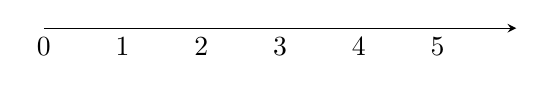
\begin{tikzpicture}
        % Draw timeline
        \draw[->,>=stealth] (0,0) -- (6,0);
        
        % Add timeline labels
        \foreach \x/\label in {0,1, 2,3, 4, 5} {
            \node[align=center, below] at (\x,0) {\label};
        }
    \end{tikzpicture}
    \caption{Timeline of Events}
\end{figure}

The sequence of events includes:
\begin{enumerate}
    \item The firm possesses knowledge of $Z,\theta,k^\alpha,e$ (where $e$ represents its endowment, different from $k$ since the firm can borrow money with $d=c+k-e$).
    \item The firm computes the optimal $k$ to maximize the expected value of the firm, with $k$ ranging from $[0,+\infty]$. If $k=0$, it indicates the firm's decision to exit.
    \item At the end of the period, the firm observes $\epsilon$ and the aggregate shock.
    \item The firm repays its debt and the fixed operating cost $(c+k-e)$, resulting in an end-of-period net worth $q$.
    \item The firm decides on the amount of dividends to distribute $(q-e')$, observes the productivity shock $\theta', Z'$, and the process restarts from step 1.
\end{enumerate}

\paragraph{Frictionless economy}
In a frictionless economy, firms have the option to borrow an amount denoted as \(c+k-e\) at the risk-free interest rate
\(r=\frac{1}{\beta}-1\). Therefore, at the start of the period, the firm's value is determined by the following
expression:

\[V_{FL} = \max_{k} E \int \max[q,\max_{e'}(q - e' + \beta V_{FL}(e',\theta', Z'))]  \,d\Phi
(\epsilon) \]
where the end of period net worth is equal to:
\[q=Z(\theta+\epsilon)k^\alpha + (1-\delta )k-(1+r)(c+k-e)\]

Under the condition of survival, it can be demonstrated that:

\[\widehat{V}_{FL}(\theta,Z) = \max_{k}E\int[Z(\theta+\epsilon)k^\alpha - (1+r)c\,d\Phi (\epsilon)] +
\beta\max[0,\widehat{V}_{FL}(\theta',Z')]\]

In the absence of market friction, firms choose to exit when their productivity reaches a certain threshold.
Specifically, they exit if \(\theta'<\underline{\theta} _{FL}(Z')\), where \(\underline{\theta}
_{FL}(Z')\) is defined as the value
for which \(\widehat{V}_{FL}(\underline{\theta}_{FL},Z')=0\).

\paragraph{Economy with Credit Market Frictions}

After production, the firm privately observes the temporary shock $\epsilon$, while financial intermediaries can only
observe it at a cost of $\mu k^\alpha$. For one-period debt contracts, financial intermediaries observe $\epsilon$ only
if the firm faces financial distress, which occurs when the private shock is insufficient to repay its debt. The terms
of the financial contract depend on the firm's net worth $e$, current productivity $\theta$, and aggregate productivity
value $Z$, all observable by both the financial intermediary and the firm at no additional cost.

\textbf{HP1 (Hypothesis 1):} The risk-free interest rate is $\beta < \frac{1}{1+r}$, which implies a lower risk-free
rate in an economy with credit frictions compared to a frictionless one. It also ensures that firms do not always
reinvest their profits.

When a firm defaults, the financial intermediary incurs verification costs and seizes all of the firm's income. The
default threshold $\overline{\epsilon}$ is determined by the equation:
\[
Z(\theta+\overline{\epsilon})k^\alpha + (1-\delta)k = (1+\widetilde{r} )(c+k+e)
\]

Default results in a zero net worth but does not necessarily force the firm to exit the market, depending on its
persistent productivity component $\theta$.

The financial intermediary lends $(c + k - e)$ to the firm only if the expected income from the loan equals the
the opportunity cost of the funds, as expressed by the inequality:
\[
(1+\widetilde{r} )(k+c+e)(1-\Phi(\overline{\epsilon}))+\int_{-\infty}^{\overline{\epsilon}}[Z(\theta+\overline{\epsilon})
k^\alpha+(1-\delta)k-\mu k^\alpha] \,d\Phi(\epsilon) \geq (1+r)(c+k+e)
\]

The financial contract is characterized by $(k,\overline{\epsilon})$. Given $Z,\theta,e$, the participation constraint
indicates the default threshold $\overline{\epsilon}$ required by the financial intermediary to lend a given amount. For
some firms, their net worth is too low for the participation constraint of the financial intermediary to be satisfied.
In fact, given $\theta, Z$, there is a unique threshold $e_b(\theta,Z)$ below which the financial intermediary
refuses to lend any amount:
\[
Z[\theta+G(\overline{\epsilon}_b )]k^\alpha+(1-\delta)k-uk_b^\alpha\Phi (\overline{\epsilon}_b)=(1+r)(k_b+c-\underline{e_b})
\]
where $\overline{\epsilon}_b$ maximizes the expected income of the financial intermediary. When the firm has a net worth
below $\underline{e_b}$, the firm defaults.

After production, the firm's end-of-period net worth is equal to:
\[
q = \begin{cases}
  Z(\theta+\overline{\epsilon})k^\alpha +(1-\delta)k-(1+\widetilde{r})(k+c-e) & \text{if } \epsilon\geq \overline{\epsilon} \\
  0 & \text{otherwise}
\end{cases}
\]
Using the default condition we can rewrite as 
\[q = \max[Zk^\alpha(\epsilon-\overline{\epsilon});0]\]

\paragraph{The firm's problem}
Define $V$ as the firm's value at the start of the period, which hinges on investment outcomes and exit decisions. If
the end-of-period net worth falls below a threshold ($q < e_b(\theta', Z')$), the firm exits. Otherwise, it compares its
continuing value to the end-of-period net worth ($q \geq e_b(\theta', Z')$) and exits if the continuing value is lower.

The firm's value function is given by:
\[
V(e,\theta,Z) = \max_{(k,\overline{\epsilon})}E\left\{\int I(q)q + (1-I(q))\max[q,\max_{e'}q-e'+\beta V(e',\theta',
\zeta')]\,d\Phi(\epsilon)\right\}
\]

Where:
\[
I(q)=
\begin{cases}
    0 & \text{if } q\geq e_b(\theta', Z')\\
    1 & \text{if } q< e_b(\theta', Z')
\end{cases}
\]

Subject to the following constraints:
\begin{enumerate}
    \item \label{con1}\[
    Z[\theta+G(\overline{\epsilon}_b )]k^\alpha+(1-\delta)k-uk_b^\alpha\Phi (\overline{\epsilon}_b)\geq(1+r)(k_b+c-
    \underline{e_b})
    \]
    \item \label{con2} \[
    q = \max[Zk^\alpha(\epsilon-\overline{\epsilon});0]
    \]
    \item \label{con3}\[
    \overline{e_b}(\theta',Z)\leq e'\leq q
    \]
\end{enumerate}

The firm aims to maximize expected dividends while complying with the financial intermediary's participation constraint
(constraint 1). Equation (constraint 2) characterizes the firm's end-of-period net worth, and
Equation (constraint 3) ensures that the
net worth
is sufficiently high to satisfy the participation constraint.
\par
Furthermore, the firm is prohibited from issuing new shares and can only augment its net worth by reinvesting profits.
This limitation presents a trade-off: increasing capital boosts production capacity but also raises the risk of default,
as the default threshold set by the financial intermediary increases with borrowed amounts.
\subsection{The cleansing effect by Caballero}

In the first paper that rationalizes the cleansing effect of recessions, \cite{CabHarm94} and published in the American Economic Review in 1994, the primary aim was to investigate how
industries respond to cyclical variations in demand. They did this by employing a vintage model of creative destruction.
The underlying concept postulates that the processes of creation and destruction within an industry partially explain
business cycles. Industries continuously experiencing creative destruction can adapt to demand fluctuations in two
ways: by adjusting the rate at which they produce new units embodying advanced techniques or by altering the
rate at which outdated units are retired. The model they used incorporated heterogeneous firms, where production units
embodied the most advanced technology at the time of their creation. The costs associated with creating new units
slowed down technology adoption, resulting in the coexistence of production units with varying vintages.
\par
Key to understanding how firms adapt to business cycles are the concepts of the creative margin and the destruction
margin. For example, a reduction in demand can be accommodated either by reducing the rate of technology adoption or by
retiring older production units. One of the primary factors determining which margin is more responsive to business
cycles is the adjustment cost. When this cost follows a linear pattern, the study shows that insulation is complete, and
the industry's response relies exclusively on its creation margin. Consequently, the creation margin becomes smoother
over time in comparison to the destruction margin, which exhibits greater responsiveness to the business cycle.
\par
Crucially, Caballero and Hammour's research \cite{BlaDia90} offers theoretical insights supported by empirical
evidence. Their findings on the cyclical nature of the destruction margin align with the studies conducted by Blanchard
and Diamond \cite{BlaDia90}, as well as Steven Davis and John Haltiwanger \cite{DavHalt92}, in their respective works
from 1990. This
convergence between theoretical framework and empirical substantiation underscores the importance of comprehending the
dynamic interplay between creative destruction and business cycles, which significantly influences how industries
respond to economic fluctuations.
\par
In their study \cite{DavHalt92}, where they assess the heterogeneity of employment changes at the establishment level in
the U.S. manufacturing sector from 1972 to 1986, it is revealed that job destruction exhibits procyclical tendencies,
responding more robustly to downturns in the economic cycle compared to the creation rate, in line with the theoretical
model proposed by Caballero and Hammour \cite{CabHarm94}. The authors leverage a natural experiment inherent in the data
to examine whether the structure of adjustment costs can account for the behavior of these two margins. This natural
experiment arises from the asymmetric nature of business cycles, with recessions being shorter but more severe than
expansions. The theoretical model predicts that these differences should be attenuated in the creation process, a
prediction that is substantiated by the data since creation exhibits relative symmetry around its mean, while
destruction displays a high degree of asymmetry.
The underlying concept driving the behavior of the destruction margin can be traced back to the theories of Schumpeter
and Hayek.  They suggest that recessions represent periods during which unprofitable or outdated techniques are pruned
from the economy, leaving behind the most efficient firms \citet{HaCa07}.
\subsection{Theoretical model}
The model in question is a vintage model that simulates an industry experiencing exogenous technological progress.
Within this model, production units are constructed using a fixed proportion of labor and capital, and they are
continually being created and phased out. Notice that only the creation of new production units
incurs a cost. This simplification is plausible, particularly in the context of the United States, where the expense
associated with hiring is typically higher than the cost of termination, as demonstrated by Abdulkadiroğlu and Kranton
(2003) \cite{AbdKra03}. 
\par
In this model, when a production unit is created at a specific time \(t_0\), it embodies the most advanced technology
available at that moment and consistently generates a uniform output represented by \(A(t_0)\) throughout its
operational lifetime. The productivity of this technology denoted as \(A(t)\), experiences continuous growth at an
exogenously determined constant rate \(\delta \ge 0 \). This growth in technology can be interpreted in two ways: either
as the adoption of new technology or as a product innovation. In the latter scenario, a continuum of perfectly
substitutable products can yield varying levels of output.

\[\left[ f(a,t) \qquad 0\leq a \leq \overline{a}(t) \right]\]

The above function represents the cross-sectional density of the production units aged \(a\) at time \(t\), where
\(\overline{a}(t)\) is the age of the oldest production unit at time \(t\). The first assumption is that \(f(a,t)\) and
\(\overline{a}(t)\) are continuous functions. The mass of production units at time \(t\) is given by:

\[N(t) = \int_{\overline{a}(t)}^{0}f(a,t)da\]

\(N(t)\) is a measure of either the industry's capital stock or its employment, due to a fixed share of capital and
labor. Thus, the industry's output is given by:

\[Q(t) = \int_{\overline{a}(t)}^{0}A(t-a)f(a,t)da\]

The deterioration of production units involves both an exogenous depreciation rate \(\delta\) and an endogenous
destruction process, which impacts \(f(a,t)\) at its limits. The count of production units surviving for \(a\) years is
expressed as: 

\[f(a,t)= f(0,t-a)e^{-\delta a} \quad \text{where } 0 < a \leq \overline{a}(t)\]

The production flow is determined by:

\[\dot{N}(t) = f(0,t) [1-\overline{\dot{a}}(t)] + \delta N(t)\]

Here, the first term represents the production rate, while the second term encapsulates the destruction rate,
encompassing the obsolescence rate \(f(\overline{a})(t)\), the technological obsolescence change over time
\(-f(\overline{a})(t)\overline{\dot{a}}(t)\), and the depreciation rate \(\delta N(t)\). 

The assumptions made by the authors are denoted as \(\forall t \mid f(0,t)>0 \cup  \overline{\dot{a}}(t)<\).

The alteration in output concerning these flows is articulated as:

\[\dot{Q}(t) = A(t)f(0,t) - A(t-\overline{a}(t))f(\overline{a}(t),t) \cdot [1-\overline{\dot{a}}(t)] + \delta Q(t)\]

The authors define a perfectly competitive industry in partial equilibrium, where supply is dictated by free entry and
perfect equilibrium. Additionally, they introduce a cost function related to creating new production units: 

\[c = c\left(f\left(f(0,t)\right)\right) \quad \text{where } c(\cdot)>0, \, c'(\cdot)\leq 0\]

This cost function is contingent on the creation rate, implying that higher creation rates correspond to increased
costs. The equilibrium condition is established by equating the cost of unit creation to the present discounted value of
profits throughout its lifespan. The authors set the cost of a production unit to 1, and \(P(t)\) is the price of a unit
of output. Thus, the profits generated at time \(t\) by a production unit aged \(a\) are defined as: 

\[\pi(a,t)= P(t)A(t-a)-1\]
\[\overline{a}[t+T(t)] = T(t)\]

Here, \(T(t)\) signifies the maximum lifetime of a unit created at \(t\). At any given time \(t\), the free entry
condition is expressed as: 

\[ c(f(0,t)) = \int_{t+T(t)}^{t}\pi(s-t,t)e^{-(r+\delta)(s-t)\,ds} \]

In the above equation, where \(r>0\) represents the exogenously determined instantaneous interest rate, the determination of
the exit of a production unit is contingent upon continuous \(P(t)\) and the instance when the profits generated by a
unit being destroyed reaches zero. This occurrence signifies the moment when the oldest unit operational at time \(t\),
denoted as \(\overline{a(t)}\), must adhere to the equation: 

\[P(t)A(t-\overline{a}(t))=1\]

The authors posit that \(P(t)\) exhibits a decreasing trend due to the model's assumption regarding endogenous
destruction, specifically \(\overline{\dot{a}(t)}<1\). To see, differentiate 
\[\dot{P}(t)=-\gamma\left[1-\overline{\dot{a}}P(t)\right]\]
Consequently, when the profits of a production unit diminish to
zero for the first time, it will be subject to destruction. 

On the demand side, the authors assume a unit-elastic demand function and consider the aggregate expenditure as
exogenous 
\(\overline{D}(t)=P(t)Q(t)\). 
The equilibrium is a path \(\left\{f(0,t),\overline{a}(t),T(t),Q(t)\right\}_{t \geq 0}\) that satisfy the following
conditions:
\begin{enumerate}
    \item \label{eq_2.1} 
        \begin{align*}
            Q(t) &= \int_{\overline{a}(t)}^{0}A(t-a)f(a,t)da
        \end{align*}
    \item \label{eq_2.2}
        \begin{align*}
            f(a,t)&=f(0,t-a)e^{-\delta a}      
        \end{align*}
    \item \label{eq_2.3}
        \begin{align*}
            T(t)&=\overline{a}\left(t+T(t)\right)        
        \end{align*}
    \item \label{eq_2.4}
        \begin{align*}
            c(f(0,t))&=\int_{t}^{t+T(t)}\left[P(s)A(t)-1\right]e^{-(r+\delta)(s-t)}\,ds
        \end{align*}
    \item \label{eq_2.5}
        \begin{align*}
            P(t)A(t-\overline{a}(t))&=1
        \end{align*}
    \item \label{eq_2.6}
        \begin{align*}
            P(t)Q(t)&=\overline{D}(t)
        \end{align*}
\end{enumerate}

The first three equations (\ref{eq_2.1}, \ref{eq_2.2}, \ref{eq_2.3}) and the fifth one (\ref{eq_2.5}) suffice to
delineate the trajectories of \(T(t)\), \(P(t)\), and \(Q(t)\), which are determined by \(\left\{f(0,t),
\overline{a}(t)\right\}\). To affirm the robustness of the conditions expressed in equations \ref{eq_2.6} and
\ref{eq_2.5}, it is possible to derive these equations as first-order conditions for the maximization of a number of
perfectly competitive firms holding production units. 

To comprehend the functioning of endogenous destruction, let's consider a scenario with constant demand. In this case,
both the destruction and creation rates change only due to supply factors. This steady state is characterized by a
constant lifetime of production units \(T(t) = \overline{a}(t) = \overline{a}^*\), resulting in a time-invariant age
distribution \(f(a,t) = f^*(a)\). Equation \ref{eq_2.5} implies that the price \(P(t)\) must consistently decrease at a
rate \(\sigma\). Higher innovation rates lead to increased productivity, raising the supply and consequently lowering
the price. Equation \ref{eq_2.2} reveals that the distribution of production units in the steady state follows a
truncated exponential distribution: 

\[f^*(a) = f^*(0)e^{-\delta a} \quad 0 \leq a \leq \overline{a}^*\]

Using free entry conditions (\ref{eq_2.4}) and the clearing condition (\ref{eq_2.6}), one can determine the creation and
destruction ages \(f^*(0)\) and \(\overline{a}^*\). Equations \ref{eq_2.1} and \ref{eq_2.5} yield the cost function and
productivity of a new production unit: 

\[\label{eq_2.7} c(f^*(0)) = \frac{e^{\gamma \overline{a}^*} - e^{-(r + \delta)\overline{a}^*}}{\gamma + r + \sigma} - \frac{1 - e^{-(r + \delta)\overline{a}^*}}{r + \delta}\]

\[\label{eq_2.8} f(0) = \frac{(\sigma + \delta)\overline{D}^*}{e^{\sigma \overline{a}^* - e^{\delta \overline{a}^*}}}\]

The authors then normalize the creation rate:

\[N = f^*(0) \cdot (1 - e^{\delta \overline{a}^*})\]

In the steady state, this is given by:

\[(9) \label{eq2.9}CC^* = \frac{\delta}{1 - e^{-\delta \overline{a}^*}}\]

Considering a special case where the creation cost is a constant \(c\), i.e., \(c(f^*(0)) = c\), substituting into
equation \ref{eq_2.7} allows retrieval of \(\overline{a}^*\). The effect of technological rate \(\sigma\) on
\(\overline{a}^*\) is decreasing, as a higher innovation rate increases the opportunity cost of delayed renovation,
while a higher cost of creating new units lowers the renovation rate. An optimal lifetime of production units increases
with higher \(r\) and \(\delta\) as it becomes harder to recover creation costs. 

Now, dropping the assumption of constant demand, we examine how the industry adjusts to demand fluctuations. Two ways
are identified in which the industry adapts production to meet demand: by reducing the rate of creation \(f(0,t)\) and
by increasing the rate of endogenous destruction \(f(\overline{a}(t),t) \cdot [1-\overline{\dot{a}}(t)]\), thus reducing
\(\overline{a}\), the age at which units are demolished. 

These two adjustments interact, leading to a reduction in demand causing the most outdated units to be scrapped,
rendering them unprofitable. However, if the recession is partially accommodated by a reduction in the creation rate,
the effect on the destruction margin is diminished. The authors argue that the extent to which creation will "insulate"
existing units from variations in demand depends on the marginal cost of creating new units \(c'f(0,t)\). When the
marginal cost of creation is zero, demand fluctuations are entirely adjusted by the creation margin. This is exemplified
in the case where \(c(f(0,t)) = c\). In such instances, the insulation effect is complete, as there is no need to retire
older units. Lowering \(f(0,t)\) is sufficient, and it is cheaper than reducing the life of existing production units. 

The insulation effect is not solely due to asymmetric adjustment costs on the creation and destruction margins. Complete
insulation would occur even with linear adjusting costs. The creation rate in the case of constant creation cost is
given by: 

\[\label{eq_2.10} f(0, t) = \frac{\dot{\bar{D}}(t) + \delta \bar{D}(t) + P(t) A(t - \bar{a}(t)) f(\bar{a}(t), t)[1 -
\dot{\bar{a}}(t)] - \dot{P}(t) Q(t)}{P(t) A(t)}\] 

In the attained equilibrium, variations in demand are entirely offset by adjustments at the creation margin denoted as
\(f(0, t)\), with \(\overline{a}(t)\) remaining steady at the destruction margin. The creation process effectively
counteracts the impact of demand fluctuations on the price \(P(t)\), effectively shielding existing units from demand
changes. The price \(P(t)\) experiences a constant decline at a rate represented by \(\sigma\), reflecting the pace of
technical progress. This consistent decline in \(P(t)\) serves as a clear signal for production units to function
optimally throughout their constant lifetime \(\overline{a}(t)^*\). \\
In the aforementioned scenario, the destruction rate is not constant, but it does not respond to demand through
variations in the age \(\overline{a}(t)^*\) at which units are destroyed. Instead, variations in the creation rates have
an impact on the number of units that reach obsolescence. If fewer units are created, fewer units become obsolete after
\(\overline{a}(t)^*\) periods. It is noteworthy that any modification leaving equations \ref{eq_2.3} to \ref{eq_2.5}
independent of \(\overline{D}(t)\) and \(f(0,t)\) does not alter the full-insulation results. 
\\
Interestingly, assumptions such as perfect competition, industry-wide return to scale, and perfect foresight are not
necessary for these conclusions. The latter is particularly noteworthy as it asserts that fully accommodating demand on
the creation side only requires knowledge of current conditions. As long as the non-negativity constraint on \(f(0,t)\)
is never binding, implementing equilibrium behaviors does not necessitate expectations of future demand. 
\subsection{Application of the model}
The model undergoes calibration utilizing Job-flow data and Industry production data. The former facilitates the
replication of job creation dynamics, while the latter is employed to mimic the behaviors of firm creation and
destruction in the manufacturing industry. To capture these dynamics, the marginal cost of creating new production units
is stipulated as positive \(c'f(0,t)\). This allows for a partial insulation effect, and the destruction margin responds
to demand fluctuations. However, introducing a dependency of \(c\) on \(f(0,t)\) compromises the analytical tractability
of the system (Equations \ref{eq_2.1} - \ref{eq_2.6}). Consequently, the authors resort to methods such as multiple
shooting to ascertain the optimal equilibrium and subsequently employ an iterative procedure to converge to the correct
expected creation rate. 

For numerical solutions, the authors adopt a linear formulation:

\[c(f(0,t))=c_0+c_1f(0,t)\]

To gain a deeper understanding of how creation and destruction respond to demand, the authors simulate sinusoidal demand
using the equation: 

\[\overline{D}(t)=1+0.07\sin(t)\]

The results are visualized in the image below, depicting the feedback of normalized creation and destruction (CC and DD)
to changes in demand. 

\begin{figure}
    \centering
    \includegraphics[scale = 0.4]{Plot2.1.png}
    \caption{Figure 1. A Creation and destruction \(c_0=0.3, c_1=1\) B Change in demand (Symmetric)}
    \label{plot:2.1}
\end{figure}

The plot clearly illustrates that the insulation effect is only partial; otherwise, DD would have remained flat, as in
the case with \(c(f(0,t)=c)\). From a mathematical perspective, destruction responds to demand as equations
\ref{eq_2.3}-\ref{eq_2.5} are no longer independent of the path \(f(0,t)\) and demand. From an economic standpoint,
increasing creation costs smoothen the creation process. In scenarios with a nearly flat innovation rate, firms during
crises cannot fully accommodate lower demand, nullifying the adoption of new production units, as the marginal costs
would exceed the reduction in existing production units. \par
In the considered model, production units integrate labor and capital in fixed proportions to generate output. Each unit
can be conceptualized as contributing to job creation within the industry, and job-flow data serves as a metric for
quantifying the flows of production units. 

Datasets that closely align with the theoretical CC and DD series have been compiled by Davis and Haltiwanger
\cite{DAvHalt90,DavHalt92} and Blanchard and Diamond \cite{BlaDia90}, drawing from various sources. The primary focus
lies on the dataset curated by Davis and Haltiwanger, who leverage the Longitudinal Research Database to construct
quarterly series for U.S. manufacturing plants spanning the period 1972:2-1986:4. 

In their empirical approach, \cite{DavHal94}utilize output to empirically determine demand, employing the growth
rate of the industrial production index as a proxy for output growth. Notably, in the foundational theoretical model,
\(Q(r)\) is smoothed by price movement, with the elasticity of demand determining the extent of smoothing, assumed to be
equal to 1. While the theoretical model maintains a constant dividend-wage, the authors acknowledge that considering
a procyclical dividend-wage, as in the case of general equilibrium with correlated industry shocks, may dampen the
effect of demand shocks. However, they assert that this adjustment would alter only the magnitude, not the direction, of
the analysis. 

The figure below illustrates the data that the model seeks to replicate, showcasing job creation, job destruction, and growth.

\begin{figure}
    \centering
    \includegraphics[scale = 0.4]{Plot2.2.png}
    \caption{Figure 1. Job creation and job destruction in U.S. Manufacturing B Index of the industrial production}
    \label{plot:2.2}
\end{figure}

To discern the characteristics of the series, the authors perform regression analysis on sectoral rates of job creation
and job destruction against leads and lags of the corresponding rates of growth. They find that job creation is less
responsive to demand fluctuations, while job destruction exhibits a more countercyclical behavior. 
\begin{figure}
    \centering
    \includegraphics[scale = 0.4]{Plot2.3.png}
    \caption{Table 2.1. Job Creation and Job Destruction in U.S. Manufacturing Response to Output Growth}
    \label{Table 2.1.}
    \footnotesize textit{Notes}: The table presents the reaction of job creation to the growth rate of the industrial
    production index. The latter is categorized into values above and below its mean (Q). The table encompasses
    quarterly observations for the two-digit SIC industries during the period 1972:2-1986:4. The coefficients are
    uniformly constrained to be equal across all sectors, with the exception of a constant (not shown).  
\end{figure}
The initial finding indicates that the rate of job destruction displays greater responsiveness to changes in sectoral
activity compared to the rate of job creation. Specifically, the sums of coefficients are -0.384 for job destruction and
0.218 for job creation showed in the table \ref{Table 2.1.}, the same results as in \cite{DAvHalt90,DavHalt92} and in
\cite{BlaDia90}.
The authors capitalize on a natural experiment rooted in the intrinsic asymmetric characteristics of business cycles.
Recessions, marked by brevity but intense contractions, provide the backdrop for the authors' model. This model
endeavors to emulate the creation rate while concurrently mitigating the impact of asymmetric cyclicality inherent in
business cycles. The empirical evidence supporting this model's behavior is encapsulated in Table \ref{Table 2.1.},
wherein two distinct scenarios are explored: output growth trajectories above \(Q^+\) and below \(Q^-\), relative to
their respective means. The table meticulously delineates how creation and destruction rates respond to these deviations
in output growth. 
\par
The salient observation emerges regarding creation rates, elucidating that they exhibit a more rapid and robust response
in instances of vigorous output growth, as opposed to scenarios where the output growth rate experiences a reduction. On
a contrasting note, the destruction margin, in line with the model's projections, manifests heightened sensitivity to a
decline in output. This responsiveness is particularly pronounced from one quarter before the onset of the shock to one
quarter after. Notably, during expansionary phases, the mean response of the destruction margin is -0.066, a notably
milder reaction compared to the recessionary case where the mean response stands at -0.634. 
\par
These empirical outcomes seamlessly align with the predictions of the model. Specifically, the creation rate exhibits
heightened responsiveness during expansionary phases, given their cyclical and symmetric nature. In contrast, the
asymmetric and non-cyclical nature of recessions triggers a more substantial decline in the production unit rate, in
line with the model's expectations. 
\par 
In order to better understand the asymmetrical behavior the authors simulate an asymmetrical demand function:
\[\cdot{\overline{D}}(t)=0.05[\cos(t)+\sin(t)] - 0.016 \sin(2t)-0.003\cos(3t)\]
\[\overline{D}(t)=1\quad r = 0.065, \delta =0.15, \gamma=0.028, c_0=0.3, c_1=1.0\] 
The results are depicted in \ref{plot:2.4}
\begin{figure}
    \centering
    \includegraphics[scale = 0.4]{Plot2.4.png}
    \caption{A.  Creation and  Destruction B. Output Growth}
    \label{plot:2.4}
    \footnotesize \textit{Notes}: The figure depicts a simulation of asymmetrical supply growth.
\end{figure}

From the plot \ref{plot:2.4}, it is evident that firms use prediction in demand to smooth job creation to avoid
big change, since they are too costly, by averaging the demand over the lifetime of a production unit. On the other
hand, destruction depends only on current conditions, thus responding only to significant deviations from the demand
prediction. It can be better understood thinking about a case in which creation rates respond only mildly to a sharp
decrease in demand, and the equilibrium price falls leading to additional destruction since older units' profits go to 0.
Indeed, destruction not only preserves but amplifies the asymmetry of demand.\paragraph{Frictionless economy}
\par
The authors culminate their study with a compelling calibration exercise using manufacturing series to exploit the
model. This entails dissecting the observed net change in employment into destruction and creation rates, as well as
applying the same approach to output production. The model is simulated for the duration of 1972:2-1983:4, with
parameters as follows: 


\begin{table}[ht]
    \centering
    \caption{Calibrated Parameters}
    \label{Tab2.1}
    \begin{tabular}{lcc}
    \hline \hline
    Variable & Symbol & Value \\
    \hline
    Interest rate & $r$ & 0.065 \\
    Depreciation rate & $\delta$ & 0.150 \\
    Rate of technical progress & $\gamma$ & 0.028 \\
    Adjustment cost parameters & $c_0$ & 0.403 \\
     & $c_1$ & 0.500 \\
    \hline
    \end{tabular}
    \end{table}
    


The technical progress is selected to attribute all the growth in employment and manufacturing to technological
advancements, setting \(\lambda\) as 2.8. The authors employ Equation \ref{eq2.9}, linking the steady state to the
lifetime of jobs and job turnover (\(CC^*\)), determining \(\overline{a}^*+7.42\) years. Utilizing this information,
they ascertain the steady state entry cost to be 0.525, equivalent to half a year's operating costs for production
units. Subsequently, they employ ordinary least squares (OLS) to retrieve the value of \(c_1\), the marginal cost of
creating a new unit, which is found to be 0.5. This aligns with a small elasticity for the creation cost function,
signifying the vulnerability of the insulation mechanism to breakdown. 
\begin{figure}
    \centering
    \includegraphics[scale = 0.6]{Plot2.5.png}
    \caption{Figure 1. A employment driven job creation \(c_0=0.403, c_1=0.5\) B Employment job destruction \(c_0=0.403, c_1=0.5\)} 
    \label{plot:2.5}
\end{figure}
The outcomes stemming from the simulations driven by employment and output are disclosed and contrasted with the data in
Figure \ref{plot:2.5}. Notably, the simulation of job creation displays a level of smoothness that diverges from the
observed 
data, with this discrepancy being attributed, in part, to the inherent absence of uncertainty in our model. Despite
this, the model effectively elucidates the relative volatility discernible in the patterns of job creation and
destruction. Moreover, it successfully captures the greater symmetry observed in the former, offering insights into the
nuanced dynamics at play in employment and output fluctuations. 
\par
The model provides intriguing insights as it elucidates certain empirical findings found in \cite{DAvHalt90,DavHalt92}.
Specifically, it delves into the dynamics of how the response of the creation margin contributes to an insulating effect
on the destruction margin. The model's salient features lie in its incorporation of heterogeneity across production
units and their turnover, rendering it a meaningful baseline for comprehending how the cleansing effect influences the
distribution of production units. 

However, it's essential to note that the model, in its current formulation, does not account for the potential impact of
financial frictions arising from asymmetric information between borrowers and lenders. Such frictions could conceivably
influence both the destruction and creation margins, introducing a layer of complexity not considered in the current
framework. 

An alternative perspective on recessions is captured by the concept of a "pit-stop," where a recession is characterized
as a period during which improvement investments in production are undertaken due to temporarily low opportunity costs,
as posited by \cite{DAvHalt90}. This viewpoint adds nuance to the understanding of recessions, emphasizing them as
periods conducive to strategic investments. 

One potential objection to the notion that recessions are times of cleansing is rooted in the implication of
countercyclical productivity. Notably, labor productivity is often observed to be procyclical. However, this apparent
inconsistency can be attributed to friction, as suggested by \cite{GaHam92}. Their findings provide evidence supporting
the notion that the cleansing effect enhances productivity in the long term, offering a nuanced perspective on the
relationship between economic downturns and productivity dynamics. 
\par
A crucial observation in the aforementioned model is the authors' reliance on a constant marginal cost of creation. Yet,
recent literature has raised concerns about the reliability of this assumption, especially for larger firms. The
dynamics of the business environment in recent years suggest that significant firms tend to favor substantial
adjustments, particularly in terms of downsizing. 
\par
Interestingly, this deviation from the constant marginal adjustment cost for bigger firms can be interpreted as a
validation of the model's predictions. When firms opt not to fully insulate themselves from a decline in demand using
the creation margin, they tend to respond with intense layoffs. This alignment between the model's predictions and the
observed behavior of larger firms underlines the model's relevance and its capacity to capture real-world dynamics. 

\section{Theoretical model}
\subsection{Introduction}
This thesis presents a partial equilibrium model in which firms maximize dividends over an infinite period, under financial frictions,
investigating how those frictions can affect the saddle paths of capital and dividends.

The subsequent sections delve into the formulation of the flow of funds and its dynamics. Following this, the focus
shifts to scenarios  where financial frictions are present, examining their
implications on firm behavior and market outcomes. %The final part of this study involves simulating the distribution of
%exiting firms in relation to their capital and productivity levels under a sinusoidal demand pattern, aiming to provide
%deeper insights into the interplay between  financial health and economic fluctuations.

\subsection{Law of motion of capital and debt}

This model is set within a partial equilibrium framework where firms are differentiated by their productivity levels.
They have the option to fund their operations by obtaining loans from financial intermediaries, as outlined by
\cite{bernanke1995inside}, or by retaining dividends. The capital at any time \(t\) is calculated by
adjusting the capital from the previous period for depreciation (\(\delta\)), then adding the net investment (\(I\)), thus the
low of motion of the capital stock is: 
\begin{align*}
    k_t &= k_{t-1}(1 - \delta)  + I_t  
\end{align*} 
The investment function is:
\begin{align}
    I_t &= k_t - k_{t-1}\left(1-\delta\right) \label{eq1}
\end{align} 
The \ref{eq1} equation states the investment level at time t is equal to the increase in capital less the depreciated ones. 
The flow of funds constraint is:
\begin{align}
    I_t + R b_{t-1} + d_t &= f(k_{t-1}) + b_t \label{eq2}
\end{align}
where \(R\) denotes the gross interest rate and \(b_{t-1}\) represents the debt from the preceding period.
The LHS of the f-of-f describes the resource outflows: 
\begin{enumerate}
    \item \(I_t\) the net investment at time t
    \item \(R b_{t-1}\) repayment of debts (capital and interest) of the previous period
    \item \(d_t\) dividends distributed at time t
\end{enumerate}
On the other hand, the RHS represents the resources inflows, which are composed by:
\begin{enumerate}
    \item \(f(k_{t-1}) \) output of production at time t
    \item  \(b_t\) debt contracted at time t
\end{enumerate}
The f-of-f constraints can be rewritten as the low of motion of debt, where \(S_t = f(k_{t-1}) - d_t\) is the retained
earnings, using \ref{eq1}, \ref{eq2}:
\begin{align*} 
    b_t &= R b_{t-1} + I_t - S_t  \label{eq2'}
\end{align*} 
The above equations state that the debt level at time t should be exactly equal to the repayment of the previous debt (capital +
interest), plus the investment net of internal funding. 
From \ref{eq1} and \ref{eq2'} follows, by definition, the low of motion of the net worth:
\begin{align*}
    n_t & = k_t- b_t = k_{t-1}(1-\delta) + I_t - R b_{t-1} - I_t + S_t \\
    &= k_{t-1} - \delta k_{t-1} - b_{t-1} - r b_{t-1}+ S_t \\
    &= n_{t-1} - \delta k_{t-1} - r b_{t-1} + \left[f\left({k_t-1}\right) - d_t \right]
\end{align*}

The net worth or equity of the firm is given by the net worth of the previous period less the depreciated capital, less
the interest matured from the previous period augmented by the retained earnings. Therefore a firm can increase its
net worth only through increasing the retained earnings levels, thus increasing output or decreasing dividends.

\paragraph{Steady State}

From \ref{eq1} we can retrieve the locus in which capital (\(k_{t-1}=k_{t}=\widehat{k}\)) and debt (\(b_{t-1}=b_{t} = \widehat{b}\))
 and  for definition even dividends (\(d_t=d_{t-1} \)):
\begin{align}
    \widehat{k}&=\widehat{k}\left(1-\delta\right) + \widehat{I}\\
    \widehat{I}&=\delta \widehat{k}  \label{eq4}
\end{align}
The \ref{eq4} stated that in the steady state, the firm will invest only to substitute depreciated capital(\(\delta \widehat{k}\)). From \ref{eq2'} substituting the stationary conditions, we get:
\begin{align}
    \widehat{b} &= R \widehat{b} + \widehat{I} - \widehat{S} \\
    \widehat{S} - \widehat{I} &= r \widehat{b} \\
    f\left(\widehat{k}\right) - \widehat{d} - \delta \widehat{k} &= r \widehat{b} \label{eq5}
\end{align}
The above equation \ref{eq5} states that in the steady state, the retained earnings should be used only to repay matured
interest over debt.
Equation \ref{eq5} can be rewritten as:
\begin{align}
    f(\widehat{k}) = \delta \cdot \widehat{k} + r \cdot \widehat{b} + \widehat{d} \label{eq5'}
\end{align}
The above equation \ref{eq5'} states that in the steady state, the production should be able to repay interest,
dividends and depreciation. 
To visualize the steady state locus, we can plot the graph \ref{fig:steadystate3d} of the locus described in the
equation \ref{eq5'} using the following production function:
\begin{align}
    f(k_{t-1}) = Z \cdot k_{t-1}^\alpha, \label{eq6} 
\end{align}
 with \(Z\) indicating the firm's productivity level, and \(k_t\) symbolizing capital as in the model by
 \cite{CabHarm94}.  

\begin{figure}
    \centering
    
    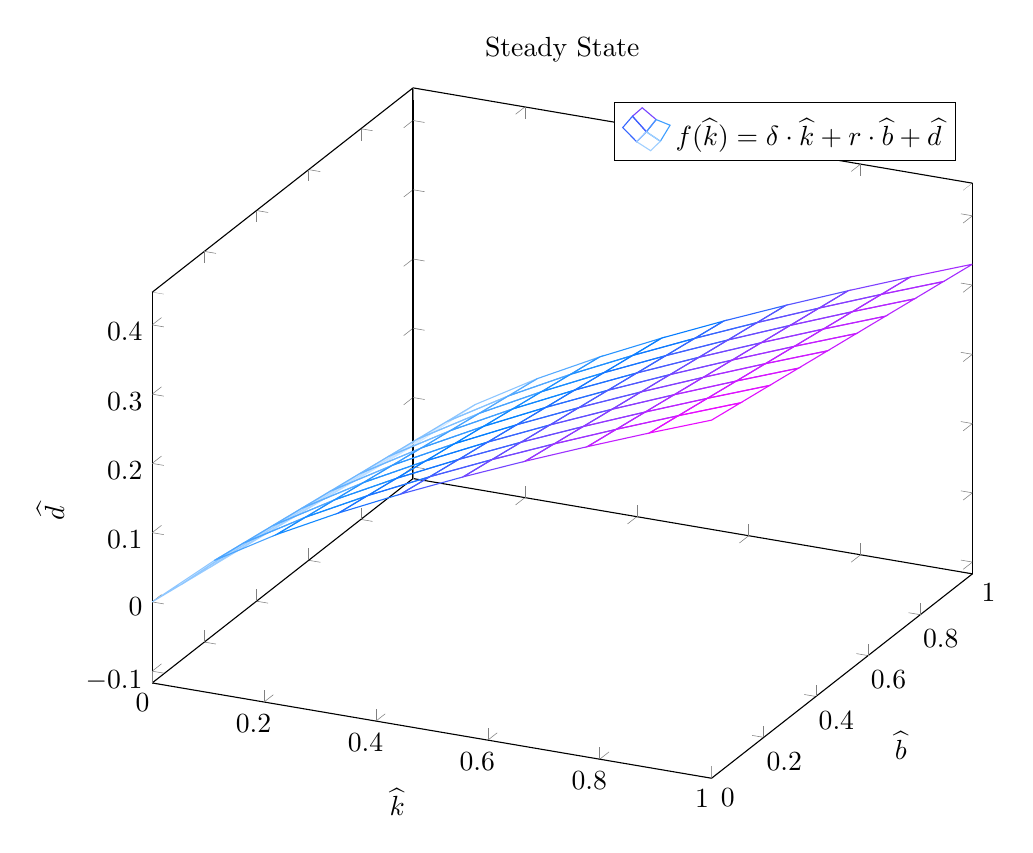
\begin{tikzpicture}
        \begin{axis}[
            title=Steady State,
            colormap/cool,
            xlabel= \(\widehat{k}\),
            ylabel= \(\widehat{b}\),
            zlabel=\(\widehat{d}\)
        ]
        \addplot3[
            mesh,
            samples=10,
            domain=0:1,
        ]
        {0.5*x^0.8-0.1*x-0.07*y};

        \addlegendentry{\(f(\widehat{k} ) = \delta \cdot \widehat{k} + r \cdot \widehat{b} + \widehat{d}\)}
        \end{axis}
    \end{tikzpicture}
    \caption{For this plot the following value has been used: \(\delta =0.1, r=0.1, \alpha=0.8, Z=0.5\)}
    \label{fig:steadystate3d}
\end{figure}

The figure illustrates the steady state relationships among debt (\(\widehat{b}\)), capital (\(\widehat{k}\)), and
dividends  (\(\widehat{d}\)) in a three-dimensional plot. The graph demonstrates how various combinations of debt and
capital influence the distribution of dividends. It is evident that increasing the level of debt results in lower
dividends, as a larger portion of resources is allocated towards servicing interest payments. Conversely, the
relationship between capital and dividends is depicted as convex, highlighting an increase in dividends with higher
capital levels, under the specified model parameters: \(\delta = 0.1\), \(r = 0.1\), \(\alpha = 0.8\), and \(Z = 0.5\).
For example, the firm starting with initial capital \(k_0 = 0.2\) and debt \(b_0 = 0.1\), to maintain a steady state for both
capital and  debt, the dividends should be equal to \(\widehat{d} = 0.5 \times 0.2^{0.8} - 0.1 \times 0.2 - 0.1
\times 0.1\). This specific combination of \(k= 0.2\), \(b = 0.1\), \(d \approx 0.11 \)represents a stationary point in the model.
\vspace{1cm}
\paragraph{Dynamics of capital}
While the discussion thus far has focused on steady states, it is crucial to explore the system's behavior under
perturbations,  particularly concerning the relationship between capital and dividends. If dividends are increased
beyond the level consistent with a stationary path—where capital remains constant over time—the analysis shifts.
Assuming the firm is debt-free (\(b_t = 0 \quad \forall t\)) for seek of simplicity, the law of motion of capital adjusts
as follows from \ref{eq2}:
\begin{align}
    I_t + d_t &= f\left(k_{t-1}\right) \quad \\
    I_t &= S_t  \label{eq7}
\end{align}
In the case of free debt, all the investment of firms is financed through internal funds as stated in the equation
\ref{eq7}. From \ref{eq7} we can retrieve the finite difference equation describing the evolution of capital:
\begin{align}
    k_{t} &= k_{t-1} (1-\delta) + f\left(k_{t-1}\right) - d_{t-1}
\end{align}
In order to understand how the above equation works, let's use the same production function as in the previous paragraph
\ref{eq6}, derive with respect to \(k_{t-1}\):
\begin{align}
    \frac{\partial{k_t}}{\partial k_{t-1}} &= \left(1-\delta\right) + f^{\prime}\left(k_{t-1}\right) \\
    \frac{\partial{k_t}}{\partial k_{t-1}} &= \left(1-\delta\right) + \alpha Z k^{\alpha-1}_{t-1}  \label{eq8}
\end{align}
There exist two cases:
if the partial derivatives with respect to \(k_{t-1}\) is greater than 1 and dividends are positive we have an exploding
path: if capital is lower than the steady state \(k_{t-1} < \widehat{k}\) the capital will shrink to 0, while in the
opposite case \(\widehat{k} < k_{t-1}\), the capital will explode to \(+\infty\). The condition for this first case is
the following:
\begin{align}
    \left(1-\delta\right) &+ \alpha Z k^{\alpha-1}_{t-1} < 1 \\
    \alpha Z k^{\alpha-1}_{t-1} &> - \left(1-\delta\right) +1 \\
    k_{t-1} &> {\frac{\delta}{\alpha Z}}^{\frac{1}{\alpha - 1}}  \label{eq9}
\end{align}
Considering the second case in which the partial derivatives with respect to \(k_{t-1}\) is less than 1 and positive
dividends, we have also an exploding path but without a steady state: for each level of capital at time t-1, the
capital at time t will be less than the previous. The condition for the latter condition is the following:
\begin{align}
    \left(1-\delta\right) &+ \alpha Z k^{\alpha-1}_{t-1} > 1 \\
    \alpha Z k^{\alpha-1}_{t-1} &< - \left(1-\delta\right) +1 \\
    k_{t-1} &< {\frac{\delta}{\alpha Z}}^{\frac{1}{\alpha - 1}} \label{eq9'}
\end{align}
The following phase diagram represent the former case \(\frac{\partial{k_t}}{\partial k_{t-1}} \leq 1\), using the following
parameters: \(\delta =
0.1\), \(r = 0.1\), \(\alpha = 0.8\), \(Z = 0.5\), and \(d = 0.8\)
\begin{figure}
    \centering
    \begin{tikzpicture}
        \begin{axis}[
            axis lines=left,
            xlabel=\(k_{t-1}\),
            ylabel={\(k_{t}\)},
            xmin=0,
            ymin=0,
        ]
        % Below the black line is defined
        \addplot [
            domain=0:5, 
            samples=100, 
            color=black,
            dotted,
        ]
        {x};
        
        % Horizontal line at y=2.5
        \draw [dotted, color=black] (axis cs:0,2.5) -- (axis cs:2.5,2.5);
        
        % Vertical line at x=2.5
        \draw [dotted, color=black] (axis cs:2.5,0) -- (axis cs:2.5,2.5);
        
        % Draw a red dot at coordinates (2.5,2.5)
        \node[draw, circle, fill=red, inner sep=2pt] at (axis cs:2.5,2.5) {};
        
        \node at (axis cs:2.5,1.8) {\(\widehat{k}\)};

        % Here the blue curve is defined with arrows
        \addplot [
            domain=0:5, 
            samples=100, 
            color=blue,
            postaction={
                decorate,
                decoration={
                    markings,
                    mark=at position 0.33 with {\arrow{<}},
                    %mark=at position 0.5 with {\arrow{>}},
                    mark=at position 0.66 with {\arrow{>}},
                }
            }
        ]
        {0.5*x^0.8 - 0.1*x + x - 0.8};
        

        \end{axis}
    \end{tikzpicture}
    \caption{The graph depicts the trajectory of capital when there is no debt involved, given the parameters \(\delta =
    0.1\), \(r = 0.1\), \(\alpha = 0.8\), \(Z = 0.5\), and \(d = 0.8\). The blue line traces the flow of funds according
    to the equation \(k_{t} = 0.5 \cdot k_{t-1}^{0.8} - 0.1 \cdot k_{t-1} + k_{t-1} - 0.8\). }

\end{figure}
The graph distinctly demonstrates that when the capital at time \(t\) is below the red dot, it signifies that the
capital is less than the steady-state capital, leading to a diminishing trajectory in the firm's capital. Conversely, if
the capital is above the steady-state level, indicated by \(\widehat{k}\), the firm is overcapitalized, and the
trajectory becomes explosive, with capital increasing without bound. 
\\
If a firm's capital is less than the steady-state, meaning it has less than the optimal amount, the outflows—such as
depreciation and constant dividends—are disproportionately high compared to its production. This dynamic will inevitably
cause the firm's capital to deplete towards zero. It's crucial to recognize that this path is predicated on the
assumption of constant dividends; the higher the dividend payout, the greater the capital necessary to ensure that
production can meet the outflows. 
\\
Furthermore, the steeper the slope of the blue line, the higher the productivity factor \(Z\), signifying a reduced need
for capital. This plays a significant role since firms with greater productivity can sustain their expenses with less
capital, which correlates with a higher likelihood of enduring economic downturns. 
\vspace{1cm}
\paragraph{Dynamics of debts}
To examine the dynamics of debt, consider a scenario where capital remains constant \(k_t=k_{t-1}=\widehat{k}\), thus it is at the
steady-state level. From equation \ref{eq5'} we get the finite difference equation for debt:
\begin{align}
    b_{t} &=  - f(\widehat{k}) + \delta \widehat{k} + R  b_{t-1} + d   \label{eq10}
\end{align}
Let's determine the condition for a stable path taking the partial derivatives with respect to \(b_{t-1}\):
\begin{align}
    \frac{\partial{b_t}}{\partial b_{t-1}} &= R  \label{eq11} \\
\end{align}
Since \(R >1\), the partial derivative \ref{eq10} will always be greater than one, thus the slope of the finite
difference equation for debt will always be steeper than one. Adding a negative intercept due to positive dividends we
get that under those conditions there exists a steady state of debt. Moreover, if the debt is below the steady state, the
debt will shrink toward 0, while if the debt is over the steady state the dynamics of debt will explode toward
\(+\infty\). This is represented in the following phase diagram:
\begin{figure}
    \centering
    \begin{tikzpicture}
        \begin{axis}[
            axis lines=left,
            xlabel=\(b_t\),
            ylabel={\(b_{t+1}\)},
            ymin=0,
            xmin=0,
        ]
        % Below the black line is defined
        \addplot [
            domain=0:5, 
            samples=100, 
            color=black,
            dotted,
        ]
        {x};
        % Horizontal line at y=2.5
        \draw [dotted, color=black] (axis cs:0,2.5) -- (axis cs:2.5,2.5);
        
        % Vertical line at x=2.5
        \draw [dotted, color=black] (axis cs:2.5,0) -- (axis cs:2.5,2.5);
        
        % Draw a red dot at coordinates (2.5,2.5)
        \node[draw, circle, fill=red, inner sep=2pt] at (axis cs:2.5,2.5) {};
        
        % Horizontal line at y=2.5
        \draw [dotted, color=black] (axis cs:0,1.1) -- (axis cs:1.1,1.1);
        
        % Vertical line at x=2.5
        \draw [dotted, color=black] (axis cs:1.1,0) -- (axis cs:1.1,1.1);
        
        
        
        % Here the blue curve is defined with arrows
        \addplot [
            domain=0:5, 
            samples=100, 
            color=blue,
            postaction={
                decorate,
                decoration={
                    markings,
                    mark=at position 0.1 with {\arrow{<}},
                    %mark=at position 0.5 with {\arrow{>}},
                    mark=at position 0.3 with {\arrow{>}},
                }
            }
        ]
        {-0.5*3^0.8 + 0.1*3 + 1.1*x + 0.8};
        % Draw a red dot at coordinates (2.5,2.5)
        \node[draw, circle, fill=green, inner sep=2pt] at (axis cs:1.1,1.1) {};

        \end{axis}
    \end{tikzpicture}
    \caption{The phase diagram illustrates the progression of debt under the condition that the change in capital (\(\Delta k\))
    is zero, with parameters set at \(\delta = 0.1\), \(r = 0.1\), \(\alpha = 0.8\), \(Z = 0.5\), \(d = 0.8\),\(\widehat{k} = 3\) . The
    blue line represents the finite difference equation for debt as modeled by the equation \(b_{t} =  - f(\widehat{k}) + \delta \cdot \widehat{k} + R
    \cdot b_{t-1} + d_{t-1}\). The red dot marks the threshold beyond which debt cannot exceed capital, effectively serving
    as a limit 
    on debt. The green dot signifies the steady state of the debt. The vertical or horizontal gap between the red and
    green dots quantifies the firm's equity. 
    }
\end{figure}
The phase diagram illustrates the relationship between a firm's current debt (\(b_t\)) and its capacity for future operations
(\(k_{t+1}\)), within the context of constant dividends. The steady state is indicated by the red dot, signifying the
juncture at which the firm's output is precisely adequate to cover dividends, depreciation, and interest on its
steady-state debt. 

If dividends were to increase, this would necessitate a higher debt level to maintain the steady state, as the firm
would have less equity. This change would be represented graphically by an elevated intercept on the curve, resulting in
an increased debt burden. 

As for productivity, firms with superior productivity require less debt to produce the same amount of dividends, as they
operate more efficiently. This is depicted by their position on the \(b_t\) axis for a given \(k_{t+1}\). However, when
the goal is to maximize dividends, highly productive firms will need more capital to reach the optimal dividend payout,
a point that will be elaborated upon while discussing the maximization problem later in the analysis. 

In essence, the graph conveys how steady-state conditions are shaped by dividend policy and productivity, with the
former influencing the firm's financial leverage and the latter determining its capital efficiency. 




\section{Free debt case: Ramsey-Cass-Kooopmans reinterpreted}
This section outlines the intertemporal maximization problem faced by the firm in the free debt case, which is a
Ramsey-Cass-Kooopmans model where there is a firm that seeks to maximize the utility of dividends instead of
consumptions levels.
The goal consists of maximizing  the present value of future dividends, formulated as:
\[V_0 = \sum_{t=0}^{+\infty}{\beta^t U(d_t)},\]
where \(U^{\prime}>0, U^{\prime \prime}<0\).
\subsection{Steady State derivation}
Consider a firm entirely financed by equity (\(b_t=0\)  for all \(t\)), leading to a simplified flow-of-funds constrant equation:
\begin{align}
    k_{t+1} = k_{t}(1 - \delta) + f(k_{t}) - d_{t}.  \label{eq13}
\end{align}
The maximization problem is tackled using a Lagrangian method, where the Lagrangian is defined as:
\[L_0 = \sum_{t=0}^{+\infty}\left[{\beta^t U(d_t) - \beta^t \lambda_t\left[k_{t+1} - k_{t}(1 - \delta) + f(k_t) - d_t\right]}\right].\]

The first-order conditions for \(d_{t}\), \(k_{t+1}\), and \(\lambda_t\) for all periods \(t=0,1,\ldots\) yield:
\[
U^{\prime}(d_{t}) = \lambda_t, \quad \forall t,
\]
\[
\beta^t \lambda_t = \beta^{t+1} \lambda_{t+1}[f^{\prime}(k_{t+1}) + (1-\delta)], \quad \forall t,
\]


This approach delineates the optimal strategy for dividend distribution and capital allocation in a debt-free
case.
In the infinite horizon model, the transversality condition reads:
$\lim _{T \rightarrow \infty} \beta^T U^{\prime}\left(d_{t}\right) k_{T+1}=0$. 
Thus, policies promoting accelerated capital accumulation are ruled out.
Differentiating  equation concerning dividend levels at time \(T+1\) yields the following set of first-order
conditions:


\begin{align}
U'(d_{t}) &= \lambda_T.
\end{align}


Each Lagrange multiplier \(\lambda_t\) represents the marginal utility of dividends in period \(t\). 

From these first-order conditions (FOCs), we derive the Euler equation for dividends:
\begin{align}
    U^{\prime}(d_{t}) = \beta U^{\prime}(d_{t+1})[f^{\prime}(k_{t+1}) + (1-\delta)]  \label{eq14}
\end{align}
indicating that the marginal utility of distributing dividends at time \(t\) should match the discounted marginal
utility of distributing  dividends in the next period, adjusted for the net marginal product of capital after accounting
for depreciation.
\paragraph{Steady state condition for dividens}
Imposing the steady state condition for dividends \( d_t = d_{t+1} = \widehat{d} \) in \ref{eq14} , we
equate the marginal  utilities across two consecutive periods:
\[U^{\prime}(d_t) = U^{\prime}(d_{t+1}):\]
\[\frac{1}{\beta} = [f^{\prime}(k_{t+1}) + (1-\delta)],\]
This condition is satisfied if:
\[f^{\prime}(k_{t+1}) = \frac{1}{\beta} - (1-\delta),\]
Let's assume that:
\begin{align}
    y_{t+2} &= Z k^{\alpha}_{t+1} = f(k_{t+1})  \label{eq15}
\end{align}
then:

\begin{align}
    f^{\prime}(k_{t+1}) &= Z \alpha k^{\alpha-1}_{t+1},  \label{eq15'}
\end{align}
From \ref{eq14} and  \ref{eq15'}, we get the steady state level of capital:
\begin{align}
    \widehat{k} &= \left[\frac{\alpha \beta Z}{1 - \beta\left(1-\delta\right)}\right]^{\frac{1}{1-\alpha}}.  \label{eq16}
\end{align}
\paragraph{steady state condition for capital}
Imposing steady state condition for capital (\(k_t = k_{t-1} = \widehat{k}\)) in the law of motion of capital \ref{eq13} we
get:
\begin{align}
    \widehat{d} & = f(\widehat{k}) - \delta \widehat{k}  \label{eq17}
\end{align}
Using the s. s. level of capital \ref{eq16} and \ref{eq15} into \ref{eq17}, we get the s.s. dividend level \(\widehat{d}\):
\begin{align}
    \widehat{d} &=Z\left[\frac{\alpha \beta Z}{1-\beta(1-\delta)}\right]^{\frac{\alpha}{1-\alpha}}-\delta\left[\frac{\alpha \beta Z}{1-\beta(1-\delta)}\right]^{\frac{1}{1-\alpha}}
     \label{eq18}
\end{align}
Thus we found the steady state level for capital and dividends.
\subsection{Phase diagram}
\paragraph{Steady state for dividends}
In this section, we will plot the phase diagram for capital and dividends exploiting steady-state conditions for capital and
dividends. 
\begin{figure}
    \centering
    \begin{tikzpicture}
        \begin{axis}[
            axis lines=middle, % sets the position of the axes
            xlabel=\(k_t\),
            ylabel=\(d_t\),
            ymin=0, xmin=0,
            xmax=5, ymax=5,
            ticks=none, % removes ticks on axes
            clip=false,
            every axis plot post/.style={thick}
        ]
        
        % Vertical line at k hat
        \draw  (axis cs:1.8,0) -- (axis cs:1.8,5);
        \node at (axis cs:2,5.5) {\(\Delta d_t = 0\)};
        \node at (axis cs:1.8,-0.5) {\(\hat{k}\)};
        
        % Arrows
        % Upwards arrows
        \draw [-{Latex[length=3mm]}] (axis cs:1,1) -- (axis cs:1,2);
    
        % Downwards arrows
        \draw [{Latex[length=3mm]}-] (axis cs:3,1) -- (axis cs:3,2);

        \end{axis}
    \end{tikzpicture}
    \caption{Phase diagram of dividends with respect to capital, depicting the steady state level for dividends.}
    \label{fig:dividend_dynamics}
\end{figure}

The graph portrays the dynamics of dividends (\(d_t\)) in relation to the capital (\(k_t\)) of a firm, with a
particular focus on the behavior when capital is below or above the steady-state level,  denoted by \(\hat{k}\).

When the capital is below the steady-state level (\(k_t < \hat{k}\)), thus on the left of the vertical line, the
firm is optimal to increase dividends over time (\(d_t<d_{t+1}\)) as represented by the arrow point upward. When instead
(\(k_t > \hat{k}\)), divdends must shrink over time (\(d_t>d_{t+1}\)).
\paragraph{Steady state for capital}
Lets look at the locus in which capital is stationary \(\Delta k = 0 \) is given by the f-of-f constraint \ref{eq17}:
\begin{align}
    \widehat{d} & = f(\widehat{k}) - \delta \widehat{k} 
\end{align}
In our case, as obtained in the above section, the locus in which capital is stationary becomes \ref{eq18}:
\begin{align}
    \widehat{d} &=Z\left[\frac{\alpha \beta Z}{1-\beta(1-\delta)}\right]^{\frac{\alpha}{1-\alpha}}-\delta\left[\frac{\alpha \beta Z}{1-\beta(1-\delta)}\right]^{\frac{1}{1-\alpha}}
\end{align}

This function starts at the origin since (\(f(0)=0\)), with a maximum in \(\underline{k}\) (defined as capital level
such that \(f^{\prime}(\underline{k})=\delta\)). From equation \ref{eq15'} we can find the level of capital that maximises dividends
at the steady state of capital:
\begin{align}
    \underline{k} &= \left[\frac{\delta}{\alpha Z}\right]  \label{eq19}
\end{align}
While \(\bar{k}\) is the capital level such that (\(d_t=0\)), thus its obtained by solving (\(f_(\bar{k}) -\delta
\bar{k} = 0\)) solving for the Cobb-Douglas production function \ref{eq15}, we get:
\begin{align}
    Z \bar{k}^{\alpha} &= \delta \bar{k}
\end{align}
\begin{figure}
    \centering
    \begin{tikzpicture}
        \begin{axis}[
            axis lines=middle, % sets the position of the axes
            xlabel=\(k_t\),
            ylabel=\(d_t\),
            xmin=0, ymin=0,
            xmax=5, ymax=5,
            ticks=none, % removes ticks on axes
            clip=false,
            axis on top=true
        ]
        
        % Parabolic curve
        \addplot [
            domain=0:4, 
            samples=100, 
            thick,
        ]
        {-x^2 + 4*x};
        
        % Vertical line at k hat

        \node at (axis cs:3.5,3.5) {\(\Delta k_t = 0\)};

        
        % Arrows on the left side
        \draw [-{Stealth[bend]}]  (axis cs:0.5,1)--(axis cs:1,1);
        \draw [-{Stealth[bend]}]  (axis cs:0.8,4) -- (axis cs:0.5,4);
        
        % Arrows on the right side
        \draw [-{Stealth[bend]}]  (axis cs:2.5,1)--(axis cs:3,1);
        \draw [-{Stealth[bend]}]  (axis cs:4,4) -- (axis cs:3.5,4);
        \node at (axis cs:2,-0.2) {\(\bar{k}\)};
        \node at (axis cs:4,-0.2) {\(\underline{k}\)};

        %vertical line at maximum
        \draw [dashed] (axis cs:2,0) -- (axis cs:2,4);
        \end{axis}
    \end{tikzpicture}
    \caption{Phase diagram of dividends concerning capital, depicting the steady state level for capital.}
\end{figure}

In the case in which a capital level \(\check{k} \in \left[0,\bar{k} \right]\), the corresponding dividends level that
guarantee the stationarity of capital is:
\begin{align}
    \check{d} &= f(\check{d}) -\delta \check{k}
\end{align}
If the firm distributes more dividends than \(\check{d}\) the capital stock must decrease over time: since the
dividends are too high the firm is consuming part of her capital. More precisely the firm is distributing more dividends than
\(\check{d}\), which guarantees that the difference between gross production, and dividends is exactly equal to capital depreciation.
This behavior is represented by the arrows above the curve pointing to the left. If the firm consumes fewer
dividends than \(\check{d}\), the opposite happens: the firm increases its capital since there is a positive net
investment. This behavior is represented by
the arrows below the curve pointing toward the right. 

\paragraph{Steady state for capital and dividend}
Merging the plot above we get a phase diagram that represents the conditions for stationarity. 
\begin{figure}
    \centering
    \begin{tikzpicture}
        \begin{axis}[
            axis lines=middle, % sets the position of the axes
            xlabel=\(k_t\),
            ylabel=\(d_t\),
            xmin=0, ymin=0,
            xmax=5, ymax=5,
            ticks=none, % removes ticks on axes
            clip=false,
            axis on top=true
        ]
        
        % Parabolic curve
        \addplot [
            domain=0:4, 
            samples=100, 
            thick,
        ]
        {-x^2 + 4*x};
        
        % Arrows
       
        
        % Vertical line at k hat
        \draw [dashed] (axis cs:2,0) -- (axis cs:2,4);
        \node at (axis cs:2.5,4.5) {\(\Delta k_t = 0\)};
        \node at (axis cs:3.5,3.5) {\(\Delta d_t = 0\)};
        \node at (axis cs:4,-0.2) {\(\underline{k} \)};

        \draw  (axis cs:1.8,0) -- (axis cs:1.8,5);

        \node at (axis cs:1.8,-0.2) {\(\hat{k} \)};
        % Arrows on the left side
        \draw [-{Stealth[bend]}]  (axis cs:1.3,1)--(axis cs:1.8,1);
        \draw [-{Stealth[bend]}]  (axis cs:0.8,3) -- (axis cs:0.3,3);
        
        % Arrows on the right side
        \draw [-{Stealth[bend]}]  (axis cs:2.5,1)--(axis cs:3,1);
        \draw [-{Stealth[bend]}]  (axis cs:4,3) -- (axis cs:3.5,3);
        
        % Arrows
        % Upwards arrows
        \draw [-{Stealth[bend]}]  (axis cs:0.8,3) -- (axis cs:0.8,3.5);
        \draw [-{Stealth[bend]}]  (axis cs:1.3,1) -- (axis cs:1.3,1.5);
        \draw [-{Stealth[bend]}]  (axis cs:2.5,1) -- (axis cs:2.5,0.5);
        \draw [-{Stealth[bend]}]  (axis cs:4,3) -- (axis cs:4,2.5);
        
        % Vertical line at k hat
        \draw [dashed] (axis cs:1,0) -- (axis cs:1,5);
        \node at (axis cs:0.8,2) {A};
        \node at (axis cs:1,-0.2) {\(k_0\)};
        \draw [dashed] (axis cs:1,0) -- (axis cs:1,5);
        
        % Draw a green dot at coordinates (1.1,1.1)
        \draw [-{Stealth[bend]}, color=blue]  (axis cs:1,2) -- (axis cs:1.76,3.87);
        \node[draw, circle, fill=green, inner sep=2pt] at (axis cs:1.81,3.96) {};
        \node[draw, circle, fill=green, inner sep=2pt] at (axis cs:1,2) {};
        \node at (axis cs:1.7,4.2) {B};
        
        \node at (axis cs:2,-0.2) {\(\bar{k}\)};
        \end{axis}
    \end{tikzpicture}
    \caption{Dynamics of consumption concerning capital accumulation, showing the points of stability and
    instability along the curve.}
\end{figure}
Notice that there exits 3 steady states: one at the origins due to the assumption \(f(0)=0\), the point \((\bar{k};0)\),
and finally point B. Point B was obtained in the previous paragraph \ref{eq16} and \ref{eq18} and represented the point in
which dividends and capital are at a steady state, and both are strictly positive (this point is also referred to as saddlepoint).
The blue line depicts a possible saddlepath towards the B. Starting at A, the firm chooses exactly the dividend level that
leads to the stationary point B. This path not only fulfills the difference equations \ref{eq14} and \ref{eq17}, but
also, the transversality condition which states:
\begin{align}
    \lim _{T \rightarrow \infty} \beta^T U^{\prime}\left(d_{t}\right) k_{T+1}=0  \label{eq20}
\end{align}
Indeed as \(t \rightarrow \infty\), capital and dividends approach their steady-state level which are both positive and
finite, thus the marginal utility of dividends at \(\hat{d}\) is also finite, hence \ref{eq20} is valid.

In conclusion, in this paragraph, we have derived the steady-state levels for both capital and dividends and plotted the
steady-state conditions in a phase diagram. In the next section, we will repeat the same exercise introducing debt and financial friction depicting  


\section{Introducing financial frictions}
In this section we tackle the infinite maximization problem of the firm, introducing the possibility of financing through
debt and two types of financial frictions. The first financial friction is a financing constraint (\(\forall t, b_t = l
k_t\)), which implies fixed leverage for the firm. The second financial friction is introducing a participation
constraint with monitoring cost \(1-\mu\) for the financial intermediaries. The goal is to understand how those frictions
affect the steady state of capital and dividends.

\subsection{Participation constraint of the financial intermediaries } 
The subsection delves into the constraints facing financial intermediaries within the model, highlighting how firms can
finance themselves either through retaining dividends or accruing debt. Initially, the model assumed an exogenous
interest rate, unaffected by the volume of debt, leading to an unrealistic scenario where interest rates remain constant
regardless of debt levels relative to equity. To address this, the model introduces a financial market where the
interest rate is determined by market-clearing conditions, and financial intermediaries operate under perfect
competition to maximize profits.

According to \cite{BerGer86}, lending should yield a profit equivalent to the opportunity cost of capital. Lenders earn
interest plus the principal if borrowers repay successfully (with probability \(p\)) or acquire the firm's production
assets (less depreciation) in case of bankruptcy. The lender's participation constraint is formulated as:
\begin{align*}
    R_t \cdot b_t p + (1-p) \mu f(k_t) = R_f b_t, \
\end{align*}

where \(r_f\) represents the risk-free rate, aligning the opportunity cost of capital with risk-free returns. This
framework allows for  the derivation of the interest rate as a function of \(p\) and \(f(k_t)\), assuming no financial
frictions and perfect information for lenders to accurately estimate recoverable amounts in all firm states.

The revised participation constraint is expressed as:
\begin{align}
    R_t=\frac{R_f}{p}  -\frac{ 1-p }{ p }\frac{\mu f(k_t)}{b_t}. \label{eq21}
\end{align}



For illustration, consider parameters \(mu = 1\), \(p = \{0.95,0.9\}\), \(\delta = 0.1\), \(\alpha = 0.8\), \(Z = 0.5\), \(d =
0.8\), \(\widehat{k} = 4\), and \(R_f=\{0.05,0.1\}\). The graphical representation suggests that as debt levels
increase, so do interest rates, reflecting the risk-return dilemma for lenders. A higher risk profile, denoted by a more
elevated red line necessitates greater returns to compensate for default risks. It's important to note that while the
the graph assumes constant capital, real-world scenarios often see debt increases leading to higher capital and,
consequently, greater production capacities. This reasoning clarifies why  the curves do not start from the origin, as
initial borrowing incorporates capital costs.
\begin{figure}
    \centering
    \begin{tikzpicture}
        \begin{axis}[
            domain=0:5, y domain=0:1.5, % Corrected the domain specification
            ymin=0, ymax=, % Set the y-axis limits
            xmin=0, xmax=5, % Set the x-axis limits
            axis lines=left,
            xlabel=\(b_t\),
            ylabel={\(r\)},
        ];
        % Below the black line is defined
        % Horizontal line at y=2.5 is outside the y-axis limit and should be removed or adjusted
        
        % Vertical line at x=2.5 is outside the y-axis limit and should be removed or adjusted
        
        % Draw a red dot at coordinates (2.5,2.5) is outside the y-axis limit and should be removed or adjusted
        
        % Horizontal line at y=1.1
        \draw [dotted, color=black] (axis cs:0,1.1) -- (axis cs:1.1,1.1);
        
        % Vertical line at x=1.1
        \draw [dotted, color=black] (axis cs:1.1,0) -- (axis cs:1.1,1.1);
        
        % Here the blue curve is defined with arrows
        \addplot [
             % Corrected the domain specification
            samples=100, 
            color=blue,
            postaction={
                decorate,
                decoration={
                    markings,
                    mark=at position 0.1 with {\arrow{>}},
                    %mark=at position 0.5 with {\arrow{>}}, % Commented out as not needed
                    mark=at position 0.3 with {\arrow{<}},
                }
            }
        ]
        {(1.1/0.90)-((0.1/0.9)*(0.5*((4)^0.8))/x)-1};

        \addplot [
             % Corrected the domain specification
            samples=100, 
            color=red,
            postaction={
                decorate,
                decoration={
                    markings,
                    mark=at position 0.1 with {\arrow{>}},
                    %mark=at position 0.5 with {\arrow{>}}, % Commented out as not needed
                    mark=at position 0.3 with {\arrow{<}},
                }
            }
        ]
        {(1.05/0.95)-((0.05/0.95)*(0.5*((4)^0.8))/x)-1};
        
        % Draw a green dot at coordinates (1.1,1.1)
        \node[draw, circle, fill=green, inner sep=2pt] at (axis cs:1.1,1.1) {};

        \end{axis}
    \end{tikzpicture}
    \caption{The figure presents a graphical analysis of the returns on loans as a function of the loan amount under a fixed capital level of 
    \(k=3\). The red curve models the scenario where the default risk probability is 
    \(1-p=0.05\)
    , implying a 5\% chance of default, while the blue curve corresponds to a higher default risk at 
    \(1-p=0.1\), a 10\% chance of default. Both curves reflect the increased interest rates required to compensate for
    the heightened risk as the debt stock grows. Notably, the opportunity cost of capital is maintained at 0.05 for the
    red one, while at 0.1 for the higher risk curve.
    }
    \label{plot:part_constraint_r_lavarge}
\end{figure}

The graph \ref{plot:part_constraint_r_lavarge} captures the dynamics between the debt stock \(b_t\) and the return on capital \(r\). An
increase in the debt stock leads to a rise in the interest rate, reflecting the augmented risk
perceived by lenders. Displayed are two distinct lines: one representing a riskier loan with a higher probability of
default and the other indicating a safer loan with a lower default probability. As anticipated, the riskier loan
scenario is characterized by a curve that lies above, dictating higher interest rates at each level of debt. The
constant capital assumption underpins this model; however, in reality, an increase in debt usually translates into an
increase in capital, thereby enhancing production potential. This factor accounts for the curves not starting at the
origin. 

Another way to visualize the participation constraint of the financial intermediaries is by defining \(x=f(k)/b\).
\begin{figure}
    \centering
    \begin{tikzpicture}
        \begin{axis}[
            domain=0:5, y domain=0:1.5, % Corrected the domain specification
            ymin=0, ymax=, % Set the y-axis limits
            xmin=0, xmax=5, % Set the x-axis limits
            axis lines=left,
            xlabel=\(f(k)/b\),
            ylabel={\(r\)},
        ];
        % Below the black line is defined
        % Horizontal line at y=2.5 is outside the y-axis limit and should be removed or adjusted
        
        % Vertical line at x=2.5 is outside the y-axis limit and should be removed or adjusted
        
        % Draw a red dot at coordinates (2.5,2.5) is outside the y-axis limit and should be removed or adjusted
        
        % Horizontal line at y=1.1
        \draw [dotted, color=black] (axis cs:0,1.1) -- (axis cs:1.1,1.1);
        
        % Vertical line at x=1.1
        \draw [dotted, color=black] (axis cs:1.1,0) -- (axis cs:1.1,1.1);
        
        % Here the blue curve is defined with arrows
        \addplot [
             % Corrected the domain specification
            samples=100, 
            color=blue,
            postaction={
                decorate,
                decoration={
                    markings,
                    % mark=at position 0.1 with {\arrow{>}},
                    % %mark=at position 0.5 with {\arrow{>}}, % Commented out as not needed
                    % mark=at position 0.3 with {\arrow{<}},
                }
            }
        ]
        {(1.1/0.90)-((0.1/0.9)*x)-1};

        \addplot [
             % Corrected the domain specification
            samples=100, 
            color=red,
            postaction={
                decorate,
                decoration={
                    markings,
                    % mark=at position 0.1 with {\arrow{>}},
                    % %mark=at position 0.5 with {\arrow{>}}, % Commented out as not needed
                    % mark=at position 0.3 with {\arrow{<}},
                }
            }
        ]
        {(1.05/0.95)-((0.05/0.95)*x)-1};
        
        % Draw a green dot at coordinates (1.1,1.1)
        \node[draw, circle, fill=green, inner sep=2pt] at (axis cs:1.1,1.1) {};

        \end{axis}
    \end{tikzpicture}
    \caption{The figure presents a graphical analysis of the returns on loans as a function of the production over the
    debt level while keeping the level of capital at
    \(k=3\). The red curve models the scenario where the default risk probability is 
    \(1-p=0.05\)
    , implying a 5\% chance of default, while the blue curve corresponds to a higher default risk at 
    \(1-p=0.1\), a 10\% chance of default. Both curves reflect the increased interest rates required to compensate for
    the heightened risk as the production-debt ratio grows. Notably, the opportunity cost of capital is maintained at 0.05 for the
    red one, while at 0.1 for the higher risk curve.
    }
    \label{plot:part_constraint_r_fixlavarge}
\end{figure}
The graph \ref{plot:part_constraint_r_fixlavarge} delineates a critical boundary within the participation constraint framework: as leverage approaches
unsustainable levels, the interest rate escalates to a certain peak, signifying a cap on the maximum interest rate that
deviates from the theoretical possibility of infinity. This ceiling on the rate is attributed to the fact that the
probability of default, denoted by \( p \), remains fixed and does not escalate alongside increasing leverage. 

Ultimately, the participation constraint internalizes the interest rate of a loan as a function of the leverage, the
opportunity cost of capital, and the default risk probability. By integrating this mechanism into the flow of funds
model, the impact of debt on capital is mediated through the variable \( r \), establishing a feedback loop where
financial leverage influences and is influenced by the cost of borrowing. 


\newpage

\subsection{Steady state and phase diagram}
 The firm's objective is to maximize its value through the optimal selection of dividends over time:

\[
\max_{{\{d_{t}\}}_{t=0}^{+\infty}}V_0 = \sum_{t=0}^{+\infty}{\beta^t U(d_t)}
\]

subject to:
\begin{enumerate}
    \item the flow of funds constraint \ref{eq2},
    \item the investment function \ref{eq1}, \
    \item the financing constraint \(b_t=l k_t \quad \forall t\)
    \item the participation constraint of borrower \ref{eq21}
\end{enumerate}
Consolidating the constraints we get the flow of funds constraints:


\begin{align}
    k_t &= \left\{k_{t-1}(1 - \delta) - \left[\frac{R_f}{p}  -\frac{ 1-p }{ p }\frac{\mu f(k_{t-1})}{l  k_{t-1}}\right] \cdot l k_{t-1} + f(k_{t-1}) - d_{t} \right \}{\left(1-l\right)}^{-1} \nonumber \\
    k_t &= \left[ \frac{1 + \mu - \mu p}{p}f(k_{t-1}) + \frac{p - \delta p - R_f l}{p} k_{t-1}  - d_{t} \right](1-l)^{-1} \label{eq:ff}
\end{align}

The Lagrangian for this optimization problem is formulated as:

\begin{align}
L=\sum_{t=0}^{+\infty}\beta^t U(d_t) - \beta^t \lambda_t\left[ \frac{1 + \mu - \mu p}{p}f(k_{t-1}) + \frac{p - \delta p - R_f l}{p} k_{t-1}  - d_{t} \right](1-l)^{-1},
\end{align}

leading to the first-order conditions for optimizing dividends and capital over time:


\begin{align}
    U'(d_t) &= \frac{\lambda_t}{\left(1-l\right)}, \quad \forall t,
\end{align}


and the dynamic optimality conditions for capital allocation:


\begin{align}
    \lambda_t = \beta \frac{\lambda_{t+1}}{\left(1-l\right)} \left[ f'(k_{t-1})\frac{1 + \mu - \mu p}{p} + \frac{p - \delta p - R_f l}{p} \right], \quad \forall t.
\end{align}


This formulation yields the Euler equation for dividends:

\begin{align}
U^{\prime}(d_{t})=\frac{\beta}{\left(1-l\right)} U^{\prime}(d_{t+1})\left[ f'(k_{t-1})\frac{1 + \mu - \mu p}{p} + \frac{p - \delta p - R_f l}{p} \right],
\end{align}

imposing (\(d_t = d_{t+1} =\hat{d}\)), we get:

\begin{align}
    \frac{\left(1-l \right) p}{\beta} &= f^{\prime}(\hat{k})\left({1+\mu-\mu p}\right) + \left({p-\delta p - R_f l}\right) \nonumber\\
    f^{\prime}(\hat{k})&=\frac{p -p l - \beta p + \beta \delta p + \beta R_f l}{\beta \left(1+\mu-\mu p\right)} \label{eq22}
\end{align}
using the Cobb Douglas production function \ref{eq15'} into \ref{eq22} we get:
\begin{align}
    Z \alpha\hat{k}^{\alpha-1} &= \frac{p -p l - \beta p + \beta \delta p + \beta R_f l}{\beta \left(1+\mu-\mu p\right)} \nonumber \\
    \hat{k} &=\left[\frac{Z \alpha \beta \left(1+\mu-\mu p\right)}{p -p l - \beta p + \beta \delta p + \beta R_f l}\right]^{\frac{1}{1-\alpha}} \label{eq23}
\end{align}
As in the free debt case, if the firm has less capital than the steady-state level \(\hat{k}\), the firm is optimal
to increase her dividends over time. When instead \(\hat{k}<k\),the firm should be better of shrinking the dividends
over time. Indeed it's easy to prove that imposing monitoring cost \(1-\mu=1\), no debt \(l=0\), and no probability of
default \(1-p=0\) we get the same capital level as in the debt-free case \ref{eq16}. Moreover its easy to see that the
steady-state capital is higher compared to the debt-free:
\begin{align*}
    \left[\frac{Z \alpha \beta (1+\mu-\mu p)}{p - p l - \beta p + \beta \delta p + \beta R_f l}\right]^{\frac{1}{1-\alpha}} &\geq \left[\frac{\alpha \beta Z}{1 - \beta(1-\delta)}\right]^{\frac{1}{1-\alpha}} \\
    \frac{(1+\mu(1-p))(1-\beta(1-\delta))}{p(1-l)+\beta(R_f l - p(1-\delta))} &\geq 0 \\
    (1+\mu(1-p))(1-\beta(1-\delta)) &\geq 0 \\
    p(1-l)+\beta(R_f l - p(1-\delta)) &\geq 0
\end{align*}
However, if we consider the case on which has no cost of monitoring \(\mu=1\) and on which has \(\mu=-.75\) ceteris
paribus, \(\hat{k}\) will be higher for the frictionless case. 

\paragraph{Steady state for capital}
Imposing s.s. condition for capital (\(k_t=k_{t+1}=\hat{k}\)) into the flow of funds constraint \ref{eq:ff}:

\begin{equation}
    \widehat{d} =\frac{1+\mu-\mu p}{p}f(\hat{k})-\left(\frac{l R_f+\delta p - l p}{p}\right)\hat{k} \label{eq:div_opt_path}
\end{equation}
It can be straightforwardly demonstrated that by setting the monitoring cost to \(1-\mu=1\), eliminating debt
with \(l=0\), and removing the risk of default by setting \(1-p=0\), we arrive at an identical level of dividends as
observed in the scenario without debt \ref{eq17}. 

The dynamics are equal to the free debt case except for the fact that the coefficient that multiplied \(f(\hat{k})\) is
higher since:
\begin{align*}
    \frac{1+\mu-\mu p}{p}&>1 \\
    1+\mu(1- p) &> p
\end{align*}
This is valid also for the coefficient of \(\hat{k}\) in equation \ref{eq:div_opt_path}, which is higher than the free
debt case:
\begin{align*}
    \frac{l R_f+\delta p - l p}{p}&>(1-\delta) \\
    \frac{l R_f+\delta p - l p}{p(1-\delta)}&>0 \\
    R_f l &> p(l-\delta)\\
    p(1-\delta)&>0
\end{align*}

\subsection{Phase diagram}
The goal of this section is to portray the phase diagram in two cases: one with monitoring costs and one without.
However, we will use a less heuristic approach compared to the phase diagram of the free debt case, using the same value
for parameters similar to \cite{OsePap17}:
\begin{table}[H]
    \centering
    \begin{tabular}{lcc}
    \hline Parameter & Symbol & Value \\
    \hline \hline
    Discount factor & $\beta$ & 0.956 \\
    Risk-free rate & $R_f$ & 1.04 \\
    Depreciation rate & $\delta$ & 0.07 \\
    Returns to scale & $\alpha$ & 0.80 \\
    Aggregate productivity & $\bar{Z}$ & 0.5 \\
    Monitoring cost & $1-\mu$ & ${0,0.75}$ \\
    Productivity &$Z$&$0.2$\\
    Probability of default & $1-p $&0.6 \\
    \hline
    \end{tabular}
    \caption{Parameters used in \cite{OsePap17}}
\end{table}
Moreover, we assume a fixed leverage of \(l=0.8\), since for the moment we want to understand the effect of monitoring
cost leaving all the other parameters equal.
\begin{figure}
    \centering
    \begin{tikzpicture}
        \begin{axis}[
            axis lines=middle, % sets the position of the axes
            xlabel=\(k_t\),
            ylabel=\(d_t\),
            xmin=0, ymin=0,
            xmax=15.5, ymax=1.3,
            % Removed ticks=none to enable ticks
            clip=false,
            axis on top=true,
            xtick={0,5,...,20}, % Adds ticks at intervals of 5 on the x-axis
            ytick={0,0.3,...,1.3}, % Adds ticks at intervals of 0.3 on the y-axis
            xticklabel style={/pgf/number format/fixed},
            yticklabel style={/pgf/number format/fixed}
        ]
        
        % Parabolic curve without monitoring costs
        \addplot [
            color=red,
            domain=0:15, 
            samples=100, 
            thick,
        ]
        {0.5*x^0.8-0.22*x};

        %optimal capital without monitoring costs
        \draw  (axis cs:6.9296,0) -- (axis cs:6.9296,0.83);
         % Parabolic curve with monitoring costs
         \addplot [
            color=blue,
            domain=0:15, 
            samples=100, 
            thick,
        ]
        {0.367*x^0.8-0.22*x};
        %optimal capital with monitoring costs
        \draw  (axis cs:2.1,0) -- (axis cs:2.1,0.2);
        
        

        \end{axis}
    \end{tikzpicture}
    \caption{This phase diagram depicts the dividends dynamics as they relate to capital. The red line corresponds to a
    firm that is carrying debt without monitoring costs, whereas the blue-line
    represents the same firm but with monitoring costs} 
    \label{pl_phase_b}
\end{figure}
% \begin{figure}
%     \centering
%     \begin{tikzpicture}
%         \begin{axis}[
%             axis lines=middle, % sets the position of the axes
%             xlabel=\(k_t\),
%             ylabel=\(d_t\),
%             xmin=0, ymin=0,
%             xmax=5, ymax=5,
%             ticks=none, % removes ticks on axes
%             clip=false,
%             axis on top=true
%         ]
        
%         % Parabolic curve
%         \addplot [
%             color=red,
%             domain=0:4, 
%             samples=100, 
%             thick,
%         ]
%         {-x^2 + 4*x};
        
%         \addplot [
%             color=blue,
%             domain=0:3.5, 
%             samples=100, 
%             thick,
%         ]
%         {-x^2 + 3.5*x};
        
%         % Arrows
       
        
%         % Vertical line at k hat
%         \draw [dashed] (axis cs:2,0) -- (axis cs:2,5);
%         \node at (axis cs:2.5,4.5) {\(\Delta k_t = 0\)};
%         \node at (axis cs:3.5,3.5) {\(\Delta d_t = 0\)};
%         \node at (axis cs:2,-0.5) {\(\underline{k} \)};

%         \draw [dashed] (axis cs:1.7,0) -- (axis cs:1.7,5);
%         \node at (axis cs:1.5,5.5) {\(\Delta k_t^{\prime} = 0\)};
%         \node at (axis cs:2.3,2) {\(\Delta d_t^{\prime} = 0\)};
%         \node at (axis cs:1.7,-0.5) {\(\underline{k}^{\prime} \)};
%         % Arrows on the left side
%         \draw [-{Stealth[bend]}]  (axis cs:1.3,1)--(axis cs:1.8,1);
%         \draw [-{Stealth[bend]}]  (axis cs:0.8,3) -- (axis cs:0.3,3);
        
%         % Arrows on the right side
%         \draw [-{Stealth[bend]}]  (axis cs:2.5,1)--(axis cs:3,1);
%         \draw [-{Stealth[bend]}]  (axis cs:4,3) -- (axis cs:3.5,3);
        
%         % Arrows
%         % Upwards arrows
%         \draw [-{Stealth[bend]}]  (axis cs:0.8,3) -- (axis cs:0.8,3.5);
%         \draw [-{Stealth[bend]}]  (axis cs:1.3,1) -- (axis cs:1.3,1.5);
%         \draw [-{Stealth[bend]}]  (axis cs:2.5,1) -- (axis cs:2.5,0.5);
%         \draw [-{Stealth[bend]}]  (axis cs:4,3) -- (axis cs:4,2.5);
        
%         % Vertical line at k hat
%         \draw [dashed] (axis cs:1,0) -- (axis cs:1,5);
%         \node at (axis cs:0.8,2) {A};
%         \node at (axis cs:1,-0.5) {\(k_0\)};
%         \draw [dashed] (axis cs:1,0) -- (axis cs:1,5);
        
%         % Draw a green dot at coordinates (1.1,1.1)
%         \draw [-{Stealth[bend]}, color=red]  (axis cs:1,2) -- (axis cs:2,4);
%         \node[draw, circle, fill=green, inner sep=2pt] at (axis cs:2,4) {};
%         \node[draw, circle, fill=green, inner sep=2pt] at (axis cs:1,2) {};
%         \node at (axis cs:2.1,4.2) {B};

%         \draw [-{Stealth[bend]}, color=blue]  (axis cs:1,1.5) -- (axis cs:1.7,3.05);
%         \node[draw, circle, fill=orange, inner sep=2pt] at (axis cs:1,1.5) {};
%         \node[draw, circle, fill=orange, inner sep=2pt] at (axis cs:1.7,3.05) {};

%         \node at (axis cs:0.8,1.5) {A'};
%         \node at (axis cs:1.8,3.15) {B'};

%         \end{axis}
%     \end{tikzpicture}
%     \caption{This diagram depicts the consumption dynamics as they relate to capital accumulation, highlighting areas of
%     stability and instability. The red line corresponds to a firm that is carrying debt, whereas the blue line
%     represents a firm with fixed leverage. The red arrow traces a potential saddle path for the indebted firm, beginning
%     from \( k_0 \), while
%      the blue arrow illustrates a conceivable saddle path for a firm with fixed leverage.} 
%     \label{pl_phase_b}
% \end{figure}
The phase diagram illustrated in \ref{pl_phase_b} depicts the capital accumulation dynamics under scenarios of fixed
leverage and varying monitoring costs. While the overall dynamics remain consistent across both scenarios, the
equilibrium capital level is notably reduced in firms that incur monitoring costs, in contrast to those without such
costs. As a result, firms with monitoring costs settle into a steady state equilibrium for dividends, which
leads to diminished dividend distributions compared to firms that do not bear these costs. 

\section{Finding optimal path}
Addressing the dynamic optimization problem with an initial condition \(k_0\), we employ a logarithmic utility function
and frame the issue through a Bellman equation:


\begin{align*}
    \max _{\{d_t\}_{t=0}^{\infty}} V_0 = \max _{\{d_t\}_{t=0}^{\infty}} \left\{U(d_0) + \beta \left[\sum_{t=1}^{\infty} \beta^{t-1} U(c_t)\right]\right\}
\end{align*}


subject to a dynamic capital accumulation constraint:

\[
k_t = \left\{k_{t-1}(1 - \delta) - \left[\frac{R_f}{p} - \frac{1-p}{p} \frac{f(k_{t-1})}{l \cdot k_t}\right] l k_{t-1} + f(k_{t-1}) - d_{t-1}\right\}(1-l)^{-1} \, \forall t.
\]

The aim is to determine the optimal dividend strategy \(d_t^*\) and the consequent capital levels \(k_{t+1}^*\) across
all periods. The optimal policy \(\varphi(.)\) links dividends and capital in a time-invariant manner, deduced from the
constraint:

\[
k_t = \left\{k_{t-1}(1 - \delta) - \frac{R_f}{p} l k_{t-1} + \frac{f(k_{t-1})}{p} - \varphi(k_{t-1})\right\}(1-l)^{-1} = \zeta(k_1).
\]

Given the continuous and differentiable nature of capital and dividends, the optimal dividend path can be represented as
a function of initial capital, thereby defining the maximum value function \(V(k_1)\) in terms of overall utility
maximization. The revised problem formulation becomes:


\begin{align}
    & V(k_0) = \max _{c_0} \left\{U(c_0) + \beta V(k_1)\right\} \\
    & \text{s.t. } k_1 = f(k_0) + (1-\delta)k_0 - c_0 \\
    & k_0 \text{ given.}
\end{align}


Before proceeding, it's critical to verify the solvability of the problem, adhering to the criteria for the existence and uniqueness of the solution: 
\begin{enumerate}
    \item \(0 < \beta < 1\),
    \item The utility function is continuous, bounded, and strictly concave,
    \item The capital transition function is concave.

\end{enumerate}


These conditions ensure the solution's uniqueness and strict concavity, although the logarithmic utility function
\(U(d_t) = \ln{d_t}\) might  not strictly meet these criteria. Utilizing alternative theorems allows for the relaxation of
the strict concavity requirement.

The optimal strategy is derived from the first order condition \(U'(d_0^*) + \beta V'(k_1) \frac{\partial k_1}{\partial d_0} = 0\), with  the  capital transition function implying \(\frac{\partial k_1}{\partial d_0} = -1\). The solution
encompasses:


\begin{align*}
    \begin{cases}
        V(k_0) = U(d_0^*) + \beta V(k_1), \\
        k_1 = \left\{k_0(1 - \delta) - \frac{R_f}{p} l k_0 + \frac{f(k_0)}{p} - d_0^*\right\}(1-l)^{-1}, \\
        U'(d_0^*) = \beta V'(k_1), \\
        k_0 \text{ given.}
    \end{cases}
\end{align*}


This system guides us towards the optimal path of dividends and capital levels, underpinning the dynamic economic analysis.

\paragraph{Guess and verify}
The method of "guess and verify" involves proposing a return function \(U(d_t) = \ln{d_t}\) and working through a
transition equation defined as \(k_1 = \left\{k_0(1 - \delta) - \frac{R_f}{p} l k_0 + \frac{f(k_0)}{p} -
d^*_0\right\}{(1-l)}^{-1}\). The first order condition (FOC) is specified as \(d_0 = [\beta V'(k_{1})]^{-1}\). When this
FOC is incorporated into the transition equation, the formulation of the problem becomes a system of equations outlined
as follows:


\begin{align*}
    \begin{cases}
        V(k_0) = \ln(d_0^*) + \beta V(k_0), \\
        k_1 = \left\{k_0(1 - \delta) - \frac{R_f}{p} l k_0 + \frac{f(k_0)}{p} - [\beta V'(k_{t+1})]^{-1} \right\}{(1-l)}^{-1}, \\
        U'(d_0^*) = \beta V'(k_1), \\
        k_0 \text{ given.}
    \end{cases}
\end{align*}


Our initial guess for the solution is:


\begin{align*}
    V(k_t) = e + f \ln{k_t},
\end{align*}


which leads to a refined system:


\begin{align*}
    \begin{cases}
        e + f \ln{k_0} = \ln{\left(\frac{k_1}{\beta f}\right)} + \beta [e + f \ln{k_1}], \\
        k_1 = \left\{k_0(1 - \delta) - \frac{R_f}{p} l k_0 + \frac{f(k_0)}{p} - \left[ \frac{k_1}{\beta f}\right] \right\}{(1-l)}^{-1}.
    \end{cases}
\end{align*}


Assuming a condition to simplify the analysis, \(p - \delta p - R_f l=0\), we solve for \(k_1\) and \(d_1\), leading to
expressions that relate capital and dividends directly to the parameters of the problem. These solutions indicate that
dividends are a proportion of the output, dependent on the firm's productivity, leverage, and risk-free rate. The
formulation highlights how dividends and capital evolve over time,  with dividends being a constant share of the
period's production.

Under conditions of no debt (\(l=0\) and thus \(p=1\)) and ignoring depreciation, we obtain simplified expressions for
capital and dividends in the steady state. This scenario suggests higher capital accumulation for a debt-free firm, as
it does not bear interest expenses. The policy function derived reflects the relationship between dividends, firm
productivity, and leverage, offering insights into the management of capital and dividends in different financial
states of a firm.

\subsection{Optimization Problem with Financial Frictions}

Following the derivation of a closed-form solution for our policy function, we now integrate financial frictions
stemming from information asymmetry between lenders and firms. We model this by introducing a discount factor \(\mu\)
on the perceived value of production, where \(0 \leq \mu \leq 1\); a value closer to 0 indicates higher friction levels.
Consequently, the lending activity modifies the optimization problem as follows:

\begin{align*}
    \max _{\left\{d_t\right\}_{t=0}^{\infty}} V_0 = \max _{\left\{d_t\right\}_{t=0}^{\infty}} \left\{ U(d_0) + \beta \left[ \sum_{t=1}^{\infty} \beta^{t-1} U(c_t) \right] \right\}
\end{align*}
subject to
\begin{align*}
    k_t = \left\{ k_{t-1}(1 - \delta) - \left[ \frac{R_f}{p} - \frac{1-p}{p} \frac{\mu f(k_{t-1})}{l \cdot k_t} \right] l k_{t-1} + f(k_{t-1}) - d_{t-1} \right\} \cdot \left(1-l\right)^{-1} \, \forall t.
\end{align*}

Adapting our approach from the frictionless scenario, we propose:
\begin{align*}
    V(k_0) = \ln(d_0^*) + \beta V(k_1),
\end{align*}
where
\begin{align*}
    k_1 = \left\{ k_0(1 - \delta) - \frac{R_f}{p} l k_0 + \frac{f(k_0)}{p} - \left[ \beta V'(k_{t+1}) \right]^{-1} \right\} \cdot \left(1-l\right)^{-1},
\end{align*}
and
\begin{align*}
    U'(d_0^*) = \beta V'(k_1).
\end{align*}

Our hypothetical solution takes the form:
\begin{align*}
    V(k_t) = e + f \ln(k_t),
\end{align*}
leading to:
\begin{align}
    e + f \ln(k_0) &= \ln\left( \frac{k_1}{\beta f} \right) + \beta \left[ e + f \ln(k_1) \right], \\
    k_1 &= \left\{ k_0(1 - \delta) - \frac{R_f}{p} l k_0 + \frac{f(k_0)}{p} - \left[ \frac{k_1}{\beta f} \right] \right\} \cdot \left(1-l\right)^{-1}.
\end{align}

Assuming \(p - \delta p - R_f l = 0\) simplifies to:
\begin{align}
    k_1 &= \left[ k_0(p - p\delta - R_f l) + \mu Z k_0^{\alpha} \right] \cdot \left( \frac{\beta f}{\beta f - l\beta f + 1} \right) p^{-1}, \\
    d_1 &= \left[ k_0(p - p\delta - R_f l) + \mu Z k_0^{\alpha} \right] \cdot \left( \frac{p}{\beta f - l\beta f + 1} \right), \\
    e + f \ln(k_0) &= \ln \left\{ \left[ k_0(p - p\delta - R_f l) + \mu Z k_0^{\alpha} \right] \cdot \left( \frac{p}{\beta f - l\beta f + 1} \right) \right\} \nonumber \\
    &\quad + \beta \left[ e + f \ln \left\{ \left[ k_0(p - p\delta - R_f l) + \mu Z k_0^{\alpha} \right] \cdot \left( \frac{\beta f}{\beta f - l\beta f + 1} \right) p^{-1} \right\} \right].
\end{align}

Hence, the transition and policy functions under financial frictions are formalized as:
\begin{align}
    k_1 &= \frac{Z \mu k_0^{\alpha} (1-\delta)}{l R_f} \frac{\alpha\beta}{1-l\alpha\beta}, \\
    d_0 &= \frac{Z \mu k_0^{\alpha} (1-\delta)}{l R_f} \frac{1-\alpha\beta}{1-l\alpha\beta} \beta, \\
    \widehat{k} &= \left[ \frac{Z \mu (1-\delta)}{l R_f} \frac{\alpha\beta}{1-l\alpha\beta} \right]^{\frac{1}{1-\alpha}}.
\end{align}

This analysis elucidates that financial frictions equate to a de facto reduction in productivity, which in turn
diminishes dividends, capital levels, and the rate at which firms accumulate capital. 

\section{Simulation Study}

To explore the distinctions between scenarios with and without financial frictions, we conduct a simulation exercise
employing  parameters consistent with those used in the \cite{OsePap17} study:

\begin{table}[H]
    \centering
    \begin{tabular}{lcc}
    \hline Parameter & Symbol & Value \\
    \hline \hline
    Discount factor & $\beta$ & 0.956 \\
    Risk-free rate & $R_f$ & 1.04 \\
    Depreciation rate & $\delta$ & 0.07 \\
    Returns to scale & $\alpha$ & 0.70 \\
    Aggregate productivity & $\bar{Z}$ & 1 \\
    Monitoring cost & $1-\mu$ & 0.25 \\
    \hline
    \end{tabular}
    \caption{Benchmark calibration}
\end{table}

Our aim is to ascertain the impact of incorporating financial frictions into the model. Therefore, we set the leverage
ratio (\(l=0.5\))  and the initial capital (\(k_0=1\)). This allows us to examine capital evolution along the optimal
path. For instance, we calculate \(p=\frac{0.5 \cdot 1.04}{1-0.07} \approx 0.559\), with the outcomes depicted in the
subsequent plots:

\begin{figure}[H]
    \centering
    \begin{tikzpicture}
    \begin{axis}[
        title={Optimal Path of Capital},
        xlabel={Time},
        ylabel={Capital},
        grid=both,
        minor tick num=1,
        major grid style={lightgray},
        minor grid style={lightgray!25},
        width=0.8\textwidth,
        height=6cm,
    ]
    \addplot[blue] table [col sep=comma, x=Time, y=Capital] {simulation.csv}; % With friction
    \addplot[red] table [col sep=comma, x=Time, y=Capital] {simulation_withoutfriction.csv}; % Without friction
    \legend{With Friction, Without Friction}
    \end{axis}
    \end{tikzpicture}
    \caption{Evolution of capital over time.}
    \label{fig:capitalEvolution}
\end{figure}

The initial plot delineates the capital's transition function:

\begin{figure}[H]
    \centering
    \begin{tikzpicture}
    \begin{axis}[
        title={Path of Dividends},
        xlabel={Time},
        ylabel={Dividends},
        grid=both,
        minor tick num=1,
        major grid style={lightgray},
        minor grid style={lightgray!25},
        width=0.8\textwidth,
        height=6cm,
    ]
    \addplot[blue] table [col sep=comma, x=Time, y=Dividends] {simulation.csv}; % With friction
    \addplot[red] table [col sep=comma, x=Time, y=Dividends] {simulation_withoutfriction.csv}; % Without friction
    \legend{With Friction, Without Friction}
    \end{axis}
    \end{tikzpicture}
    \caption{Evolution of dividends over time.}
    \label{fig:dividendsEvolution}
\end{figure}

It is apparent that the trajectory of dividends is consistently higher in scenarios devoid of financial frictions,
underscoring the impact of such frictions on diminishing returns. This comparison vividly demonstrates the differential
outcomes in capital and dividend paths under varying financial conditions, highlighting the broader implications of
financial frictions on economic performance and firm-level profitability. 

\subsection{heterogeneity and Aggregation Mechanism}

To refine our model, we introduce heterogeneity among firms, marking a departure from uniform productivity and leverage
ratios.  Specifically, productivity levels (\( Z_i \)) now vary across firms, introducing a spectrum of efficiency within
the model. Additionally, we diversify leverage ratios, ensuring no direct correlation between a firm's productivity and
its leverage. This heterogeneity is captured from the outset by simulating the initial distribution of capital,
leverage, and productivity, setting the stage for a dynamic interplay of firm characteristics. The aggregate production
is then represented as:
\[
\overline{K} = \int_{\underline{K} }^{\overline{k} }Z_i k_{i,t}^{\alpha}\,di
\]

Business cycles impact capital fluctuations, with each firm's changes being proportional to its existing capital. Less
efficient firms endure more significant reductions during economic downturns, while all firms enjoy capital increases
during upswings. Market exit is modeled through two avenues: voluntary exit for returns on equity below the risk-free
rate, and bankruptcy due to failure to cover debts and depreciation. The model incorporates a sinusoidal business
cycle affecting output as follows:
\[
\Delta \overline{K}_t = 1 + 0.05 \sin(t)
\]

Productivity (\( Z \)) and leverage (\( l \)) follow truncated normal distributions:
\begin{align}
    l &\sim \mathcal{N}(0.05, 0.1), \quad 0.01 \leq l \leq 1, \\
    Z-1 &\sim \mathcal{N}(0.5, 0.1), \quad 1.01 \leq Z \leq 1.1.
\end{align}

The figure below demonstrates the results of a 20-step simulation for 10 firms, contrasting optimal and actual capital
levels.  The actual capital adjusts in response to the business cycle:
\[
\Delta \overline{K}_t = 1 + 0.05 \sin(t)
\]

\begin{figure}[H]
    \centering
    \includegraphics[scale=0.4]{OptimalK_noexit.png}
    \caption{Illustrating a 20-step simulation of 10 firms, this plot compares the chosen optimal capital (\(k\))
    against the
     actual capital (\(k\)) post-business cycle adjustment.}
    \label{fig:optKnoE}
\end{figure}

Following this, the distribution of dividends, based on actual capital, is visualized:
\begin{figure}[H]
    \centering
    \includegraphics[scale=0.4]{div_cap_noexit.png}
    \caption{Displaying a 20-step simulation for 10 firms, this plot highlights dividends (\( d \)) and the actual capital
    (\(k\)) after business cycle
     adjustments.}
    \label{fig:divNoExit}
\end{figure}

Figure \ref{fig:divNoExit} distinctly shows that firms with superior productivity yield higher dividends. Moreover, upon
achieving a steady state, both capital and dividends exhibit oscillations around a rising mean. 
\begin{figure}[H]
    \centering
    \includegraphics[scale=0.4]{Output_noexit.png}
    \caption{Showcasing a 20-step simulation of 10 firms, this plot reveals the adjusted output (\( K \)) following the business cycle impact.}
    \label{fig:OutNoExit}
\end{figure}


\subsection{The Exit Mechanism}

A firm is prompted to exit the market if its return on capital ranks as the lowest within the firm distribution, making
way for a newcomer who inherits the minimum capital from the existing pool. Subsequently, the exiting firm's capital is
reallocated proportionally among the remaining firms, based on their respective returns on capital. The return on
capital for firm \( i \) at time \( t \) is defined as: 
\[
R_{i,t} = \frac{d_{i,t}}{k_{i,t}}
\]
Should a firm exhibit the \( \min{R} \), it is compelled to exit the market due to possessing the lowest return on capital
among all firms.\footnote{This criterion is enforced at each step, effectively merging the concepts of reallocation and
exit mechanisms henceforth.} 

In the ensuing simulation, while all parameters remain consistent with prior examples, the distinctive feature now is
the market exit of firms. The subsequent figure illustrates both the optimal and actual capital paths for each firm: 

\begin{figure}[H]
    \centering
    \includegraphics[scale=0.4]{OptimalK_exit.png}
    \caption{Displaying a 20-step simulation involving 10 firms: the optimal \( k \) represents the firm's capital choice,
    whereas the actual \( k \) reflects capital post-adjustment for the business cycle
     effect.}
    \label{fig:optKE}
\end{figure}

Contrasting with previous outcomes, the introduction of an exit mechanism and the redistribution of residual
capital—proportionate to returns, yet ensuring the new entrant retains the minimum capital from the firm
distribution—markedly influences capital trajectory. These mechanisms facilitate incumbent firms in accruing additional
capital, thus hastening their approach to a stationary state, particularly benefiting the most productive entities. This
dynamic underscores the cleansing effect of recessions, as capital reallocation during economic downturns favors
business continuity. The impact of reallocation manifests in the subsequent graph, which delineates a higher
dividends trajectory compared to scenarios devoid of reallocation mechanisms: 

\begin{figure}[H]
    \centering
    \includegraphics[scale=0.4]{div_cap_exit.png}
    \caption{This figure showcases the results of a 20-step simulation with 10 firms, highlighting dividends (\( d \))
    and actual 
    capital (\( k \)) following business cycle adjustments.}
    \label{fig:divExit}
\end{figure}

Ultimately, examining overall production reveals an uptick attributable to capital reallocation when juxtaposed with
prior simulations, underscoring the efficiency of the exit and reallocation strategies in fostering economic resilience
and growth.


\begin{figure}[H]
    \centering
    \begin{tikzpicture}
    \begin{axis}[
        title={Path of Overall Output},
        xlabel={Time},
        ylabel={\( K \)},
        grid=both,
        minor tick num=1,
        major grid style={lightgray},
        minor grid style={lightgray!25},
        width=0.8\textwidth,
        height=6cm,
    ]
    \addplot[blue] table [col sep=comma, x=Step, y=Total Production] {exit_nofrictions.csv}; % Blue line for exit mechanism
    \addplot[red] table [col sep=comma, x=Step, y=Total Production] {noexit_nofrictions.csv}; % Red line for no exit mechanism
    \legend{With Exit Mechanism, Without Exit Mechanism}
    \end{axis}
    \end{tikzpicture}
    \caption{This plot illustrates a 20-step simulation involving 10 firms and demonstrates the impact of business cycle
    adjustments on overall output \( K \). The blue line represents the scenario incorporating an exit mechanism, whereas
    the red line denotes the scenario without an exit mechanism, illustrating the variations in output across both
     contexts.}
    \label{fig:OutExit}
\end{figure}

Integrating the exit and reallocation mechanisms notably enhances both the dividends' trajectory and the aggregate
output, distinctly highlighting how the cleansing effect bolsters productivity. 


\subsection{Incorporating Financial Frictions into the Model}


In keeping with the methodology set forth in \cite{OsePap17}, financial frictions are incorporated into the model,
parameterized as  \(1-\mu = 0.25\). To discern the cleansing effect amidst financial frictions, an initial simulation is
run where capital remains static due to the absence of a reallocation or exit mechanism. Subsequently, a contrasting
simulation is performed where capital reallocation is possible, with both iterations subjected to financial frictions.

The following plot illustrates the progression of total output over time, displaying two distinct scenarios. The red
line delineates the case without financial frictions, and the blue line portrays the scenario with frictions in place.

\begin{figure}[H]
    \centering
    \begin{tikzpicture}
    \begin{axis}[
        title={Path of Overall Output},
        xlabel={Time},
        ylabel={K},
        grid=both,
        minor tick num=1,
        major grid style={lightgray},
        minor grid style={lightgray!25},
        width=0.8\textwidth,
        height=6cm,
        legend entries={Without Frictions,With Frictions},
        legend style={at={(0.5,-0.2)},anchor=north,legend cell align=left}
    ]
    \addplot[red, mark=square*] table [col sep=comma, x=Step, y=Total Production] {noexit_frictions.csv};
    \addplot[blue, mark=otimes*] table [col sep=comma, x=Step, y=Total Production] {exit_frictions.csv};
    \end{axis}
    \end{tikzpicture}
    \caption{Evolution of the overall output over time. The red line represents the scenario without reallocation and
    exit mechanisms, 
     while the blue line represents the scenario with these mechanisms under financial frictions.}
    \label{fig:output_evolution_frictions}
\end{figure}

Observations indicate that financial frictions attenuate overall production, akin to an effective reduction in
productivity when  firms operate with leverage. Although the cleansing effect is evident without financial frictions, it
is imperative to examine whether this effect is sustained when frictions are introduced. To this end, the subsequent plot
juxtaposes the overall output for two comparable financial friction scenarios: one with capital reallocation and one
without.

\begin{figure}[H]
    \centering
    \begin{tikzpicture}
    \begin{axis}[
        title={Path of Overall Output with Financial Frictions},
        xlabel={Time},
        ylabel={K},
        grid=both,
        minor tick num=1,
        major grid style={lightgray},
        minor grid style={lightgray!25},
        width=0.8\textwidth,
        height=6cm,
        legend entries={Reallocation Allowed,No Reallocation},
        legend style={at={(0.5,-0.2)},anchor=north,legend cell align=left}
    ]
    \addplot[blue, mark=*] table [col sep=comma, x=Step, y=Total Production] {exit_frictions.csv};
    \addplot[red, mark=x] table [col sep=comma, x=Step, y=Total Production] {noexit_frictions.csv};
    \end{axis}
    \end{tikzpicture}
    \caption{Comparison of overall output with financial frictions over time. The blue line illustrates the output when
    reallocation  
    is allowed, while the red line indicates the output when it is not.}
    \label{fig:output_comparison_frictions}
\end{figure}
Figure \ref{fig:output_comparison_frictions} demonstrates that, even under financial frictions where \(1- \mu =0.25\),
there is a productivity-enhancing mechanism facilitated by capital reallocation due to firm exits. This occurs despite
the presence of asymmetric information between financial intermediaries and firms, as discussed in \cite{OsePap17}.
Furthermore, the cleansing effect on overall production appears to be cumulative, with its impact amplifying over time,
as evidenced by the trend in the graph. Thus, it can be concluded that two economies, identical in their distribution of
productivity and capital among firms and initialized with the same seed\footnote{All simulations were conducted with the
the same seed for consistency.}, will diverge in terms of output and productivity if one allows for capital reallocation
through firm exits. This divergence is not only distinct but also grows as time progresses. 

\section{Solving the Belman with Benveniste-Scheinkman}
In this section, I will address the intertemporal maximization problem without the assumption of fixed leverage,
utilizing the Benveniste-Scheinkman equation to derive the functional form of the solution. This approach aims to
demonstrate that the optimal capital trajectory does not significantly deviate from the results obtained in the prior
analysis. However, I will refrain from conducting simulations using the policy function derived through this method, as
it yields only a series of optimal paths rather than a comprehensive simulation framework. 

\[V(k_{t}) = \max_{k_{t+1}, e_{t+1}} d_t + \beta V(k_{t+1})\]
\[s.t.\]
\[f(k_t) = Z k_t^\alpha\]
\[f(k_t) = d_t + (c+k_{t-1}-e_{t-1})(1+r) + k_{t} - (c + k_{t}- e_{t}) - k_{-1}(1-\delta)\]
\[(1+r)(c+k_t -e_t)p + (1-p)f(k_t) = (1+r_f)(c+k_t -e_t) \]
\[B_t = c+k_t-e_t; R= 1+r; R_f= 1 + r_f;  \]
\[R=\frac{R_f}{p}  -\frac{ 1-p }{ p }\frac{f(k_t)}{D_t}\]
To understand the mechanism behind this optimization problem, I first solve the three times problem working
backward.
The value function in \(t=2\) is 
\[ V_{t+2} =  \max d_{t+2}\]
Since there firm will not exists in t+2, there are no investment \(B_{t+2}=0\), thus \(0=k_{t+2}+c-e_{t+2}\) as
consequence \(k_{t+2} = e_{t+2} - c\). Then we can rewrite the value function:
\[ V_{t+2} = \max Z(e_{t+2} - c)^\alpha - (c+k_{t+1}-e_{t+1})(1+r_{t+1}) - e_{t+2} + c + (c + e_{t+2} - c - e_{t+2}) +
k_{t+1}(1-\delta) \]
\[V_{t+2} = \max_{e_{t+2}} Z(e_{t+2} - c)^\alpha - B_{t+1}R_{l,t+1} - e_{t+2} + c + k_{t+1}(1-\delta) \]
FOC:
\[\frac{\partial V_{t+2}}{\partial e_{t+2}} = Z \alpha (e_{t+2} - c)^{\alpha-1} - 1 = 0\]
\[ (e_{t+2} - c)^{\alpha-1}= (Z \alpha)^{-1}\]
\[ e_{t+2} = (Z \alpha)^{\frac{1}{1-\alpha}}+c\]
Thus:
\[d_{t+2} = Z\left[(Z \alpha)^{\frac{\alpha}{1-\alpha}}\right]  - B_{t+1}R_{t+1} -  \left[(Z
\alpha)^{\frac{1}{1-\alpha}}\right] + k_{t+1}(1-\delta) \]
\[V_{t+2} = Z\left[(Z \alpha)^{\frac{\alpha}{1-\alpha}}\right]  - B_{t+1}R_{t+1} -  \left[(Z
\alpha)^{\frac{1}{1-\alpha}}\right] + k_{t+1}(1-\delta) \]
Writing the problem in t+1:
\[V_{t+1} = \max_{e_{t+1},k_{t+1}} d_{t+1} + \beta V_{t+2}\]
\[d_{t+1} = Zk^\alpha_{t+1} - B_t R_L - k_{t+1} + B_{t+1} + k_t(1-\delta)\]
FOCs:
\begin{align*}
    \left\{\begin{array}{@{}l@{}}
        \frac{\partial V_{t+1}}{\partial e_{t+1}} = \frac{\partial d_{t+1}}{\partial e_{t+1}} + \beta \frac{\partial
            V_{t+2}}{\partial e_{t+1}} = 0  \\
        \frac{\partial V_{t+1}}{\partial k_{t+1}} = \frac{\partial d_{t+1}}{\partial k_{t+1}} + \beta \frac{\partial
            V_{t+2}}{\partial K_{t+1}} = 0 \\
    \end{array} \right .\,
\end{align*}
solving \(\frac{\partial d_{t+1}}{\partial e_{t+1}}\):
\[\frac{\partial d_{t+1}}{\partial e_{t+1}} = Z \alpha k_{t+1} ^{\alpha-1}\frac{\partial k_{t+1}}{\partial e_{t+1}}
 - \frac{\partial k_{t+1}}{\partial e_{t+1}} + \frac{\partial B_{t+1}}{\partial e_{t+1}}\]
\[\frac{\partial B_{t+1}}{\partial e_{t+1}} = \frac{\partial k_{t+1}}{\partial e_{t+1}} - 1\]
\[\frac{\partial d_{t+1}}{\partial e_{t+1}} = Z \alpha k_{t+1} ^{\alpha-1}\frac{\partial k_{t+1}}{\partial e_{t+1}} -
\frac{\partial k_{t+1}}{\partial e_{t+1}} + \frac{\partial k_{t+1}}{\partial e_{t+1}} - 1\]

solving \(\frac{\partial V_{t+2}}{\partial e_{t+1}}\):
\[\frac{\partial V_{t+2}}{\partial e_{t+1}} = - \left[\frac{\partial B_{t+1}R_{t+1}}{\partial e_{t+1}} - \frac{\partial
k_{t+1}}{\partial e_{t+1}} \left( 1-\delta \right) \right]\] 
\[\frac{\partial B_{t+1}R_{t+1}}{\partial e_{t+1}} = \frac{\partial B_{t+1}}{\partial e_{t+1}}R_{t+1} +
B_{t+1}\frac{\partial R_{t+1}}{\partial e_{t+1}} \]
\[\frac{\partial B_{t+1}}{\partial e_{t+1}} = \frac{\partial k_{t+1}}{\partial e_{t+1}}-1\]
\[\frac{\partial R_{t+1}}{\partial e_{t+1}} = - \frac{1-p}{p}\left\{\left[Z\alpha k^{\alpha-1}_{t+1}\frac{\partial
k_{t+1}}{\partial e_{t+1}} -\delta \frac{\partial k_{t+1}}{\partial e_{t+1}}\right] B_{t+1} - \left(\frac{\partial
k_{t+1}}{\partial e_{t+1}} - 1\right) \left[Zk_{t+1}^{\alpha} - \delta k_{t+1}\right]\right\}B_{t+1}^{-2}\]
\[\frac{\partial B_{t+1}R_{t+1}}{\partial e_{t+1}} = \left[\frac{\partial k_{t+1}}{\partial e_{t+1}}-1 \right] R_{t+1}
- \frac{1-p}{p}\left\{\left[Z\alpha k^{\alpha-1}_{t+1}\frac{\partial
k_{t+1}}{\partial e_{t+1}} -\delta \frac{\partial k_{t+1}}{\partial e_{t+1}}\right] B_{t+1} - \left(\frac{\partial
k_{t+1}}{\partial e_{t+1}} - 1\right) \left[Zk_{t+1}^{\alpha} - \delta k_{t+1}\right]\right\}B_{t+1}^{-1}\]
\[\frac{\partial B_{t+1}R_{t+1}}{\partial e_{t+1}} = \left(\frac{\partial k_{t+1}}{\partial e_{t+1}} -1
\right)\left[\left(zk^\alpha_{t+1} -\delta k_{t+1}\right)\frac{1-p}{p}B_{t+1}^{-1}+R_{t+1}\right] -
\frac{1-p}{p}\frac{\partial k_{t+1}}{\partial e_{t+1}} \left(Z\alpha k^{\alpha-1}_{t+1} - \delta\right)\]
\[\frac{\partial B_{t+1}R_{t+1}}{\partial e_{t+1}} = \left(\frac{\partial k_{t+1}}{\partial e_{t+1}} -1
\right)R_f-
\frac{1-p}{p}\frac{\partial k_{t+1}}{\partial e_{t+1}} \left(Z\alpha k^{\alpha-1}_{t+1} - \delta\right)\]
\[\frac{\partial V_{t+2}}{\partial e_{t+1}} = - \left[\left(\frac{\partial k_{t+1}}{\partial e_{t+1}} -1
\right)R_f-
\frac{1-p}{p}\frac{\partial k_{t+1}}{\partial e_{t+1}} \left(Z\alpha k^{\alpha-1}_{t+1} - \delta\right) - \frac{\partial
k_{t+1}}{\partial e_{t+1}} \left( 1-\delta \right)\right]\]
Substituting into the first FOC, we get:
\[\frac{\partial V_{t+1}}{\partial e_{t+1}} = Z \alpha k_{t+1} ^{\alpha-1}\frac{\partial k_{t+1}}{\partial e_{t+1}} -
\frac{\partial k_{t+1}}{\partial e_{t+1}} + \frac{\partial k_{t+1}}{\partial e_{t+1}} - 1 - \beta 
\left[\left(\frac{\partial k_{t+1}}{\partial e_{t+1}} -1 
\right)R_f-
\frac{1-p}{p}\frac{\partial k_{t+1}}{\partial e_{t+1}} \left(Z\alpha k^{\alpha-1}_{t+1} - \delta\right) - \frac{\partial
k_{t+1}}{\partial e_{t+1}} \left( 1-\delta \right)\right] = 0\]
second FOC: \\
solving \(\frac{\partial d_{t+1}}{\partial k_{t+1}}\):
\[\frac{\partial d_{t+1}}{\partial k_{t+1}} = Z \alpha k_{t+1} ^{\alpha-1} - 1 + \frac{\partial B_{t+1}}{\partial
k_{t+1}} \]
\[\frac{\partial B_{t+1}}{\partial
k_{t+1}} = 1 - \frac{\partial e_{t+1}}{\partial k_{t+1}} \]
\[\frac{\partial d_{t+1}}{\partial k_{t+1}} = Z \alpha k_{t+1} ^{\alpha-1} - \frac{\partial e_{t+1}}{\partial
k_{t+1}}\]
solving \(\frac{\partial V_{t+2}}{\partial k_{t+1}}\):
\[\frac{\partial V_{t+2}}{\partial k_{t+1}} = -\left[\frac{\partial B_{t+1}R_{t+1}}{\partial k_{t+1}} -(1-\delta)\right] \]
\[\frac{\partial B_{t+1}R_{t+1}}{\partial k_{t+1}} = \frac{\partial B_{t+1}}{\partial k_{t+1}}R_{t+1} +
B_{t+1}\frac{\partial R_{t+1}}{\partial k_{t+1}}\]
\[\frac{\partial B_{t+1}}{\partial k_{t+1}} = 1-\frac{\partial e_{t+1}}{\partial k_{t+1}} \]
\[\frac{\partial R_{t+1}}{\partial k_{t+1}} =  - \frac{1-p}{p}\left[\left(Z\alpha k^{\alpha-1}_{t+1}-\delta\right)B_{t+1} -
\left(1-\frac{\partial e_{t+1}}{\partial k_{t+1}}\right)\left(Zk_{t+1}^{\alpha} - \delta k_{t+1}
\right)\right]B_{t+1}^{-2} 
\]
\[\frac{\partial B_{t+1}R_{t+1}}{\partial k_{t+1}} = \left(1-\frac{\partial e_{t+1}}{\partial k_{t+1}}\right) R_{t+1} +
\left\{\frac{1-p}{p}\left[(Z \alpha k^{\alpha-1}_{t+1}-\delta)B_{t+1} -
\left(1-\frac{\partial e_{t+1}}{\partial k_{t+1}}\right)\left(Zk_{t+1}^{\alpha} - \delta k_{t+1}
\right)\right]B_{t+1}^{-1} \right\}\]
\[\frac{\partial B_{t+1}R_{t+1}}{\partial k_{t+1}} =\left(1-\frac{\partial e_{t+}}{\partial k_{t+1}}\right)
\left[R_{t+1} + \frac{1-p}{p}\left(Z k_{t+1}^{\alpha} - \delta k_{t+1}\right)B_{t+1}^{-1}\right]-
\frac{1-p}{p}\left(Z\alpha k^{\alpha-1}_{t+1}-\delta\right) \]
\[\frac{\partial B_{t+1}R_{t+1}}{\partial k_{t+1}} =\left(1-\frac{\partial e_{t+1}}{\partial k_{t+1}}\right)
R_f - \frac{1-p}{p}\left(Z\alpha k^{\alpha-1}_{t+1}-\delta\right) \]
\[\frac{\partial V_{t+2}}{\partial k_{t+1}} = -\left[\left(1-\frac{\partial e_{t+1}}{\partial k_{t+1}}\right)
R_f - \frac{1-p}{p}\left(Z\alpha k^{\alpha-1}_{t+1}-\delta\right)- \left(1-\delta\right)\right] \]
Substituting into the FOC:
\[\frac{\partial V_{t+1}}{\partial k_{t+1}} =Z \alpha k_{t+1} ^{\alpha-1} - \frac{\partial e_{t+1}}{\partial
k_{t+1}} - \beta \left[\left(1-\frac{\partial e_{t+1}}{\partial k_{t+1}}\right)
R_f - \frac{1-p}{p}\left(Z\alpha k^{\alpha-1}_{t+1}-\delta\right)- \left(1-\delta\right)\right]=0\]
thus the FOCs are:
\[\frac{\partial V_{t+1}}{\partial e_{t+1}} = Z \alpha k_{t+1} ^{\alpha-1}\frac{\partial k_{t+1}}{\partial e_{t+1}}  - 1 - \beta 
\left[\left(\frac{\partial k_{t+1}}{\partial e_{t+1}} -1 
\right)R_f-
\frac{1-p}{p}\frac{\partial k_{t+1}}{\partial e_{t+1}} \left(Z\alpha k^{\alpha-1}_{t+1} - \delta\right) - \frac{\partial
k_{t+1}}{\partial e_{t+1}} \left( 1-\delta \right)\right] = 0\]
\[\frac{\partial V_{t+1}}{\partial k_{t+1}} =Z \alpha k_{t+1} ^{\alpha-1} - \frac{\partial e_{t+1}}{\partial
k_{t+1}} - \beta \left[\left(1-\frac{\partial e_{t+1}}{\partial k_{t+1}}\right)
R_f - \frac{1-p}{p}\left(Z\alpha k^{\alpha-1}_{t+1}-\delta\right)- \left(1-\delta\right)\right]=0\]
rearranging \(\frac{\partial V_{t+1}}{\partial k_{t+1}} \) to isolate \(k_{t+1}\):
\[k^{\alpha-1}_{t+1}=\left[\frac{\partial e_{t+1}}{\partial k_{t+1}}\left(1-\beta R_f\right) + \beta
\left(r_f+\frac{\delta}{p}\right)\right]\left\{Z\alpha\left[\left(1-\beta\right)-\frac{\beta}{p}\right]\right\}^{-1}\] 
rearranging \(\frac{\partial V_{t+1}}{\partial e_{t+1}} \) to isolate \(k_{t+1}\):
\[k^{\alpha-1}_{t+1}=\left[\frac{\partial k_{t+1}}{\partial e_{t+1}}\left(1-\beta R_f\right) + \beta
\left(r_f+\delta\right) + \delta \frac{1-p}{p}\right]\frac{p}{Z\alpha}\]
Equating the two equations:
\[\left[\frac{\partial e_{t+1}}{\partial k_{t+1}}\left(1-\beta R_f\right) + \beta
\left(r_f+\frac{\delta}{p}\right)\right]\left\{Z\alpha\left[\left(1-\beta\right)-\frac{\beta}{p}\right]\right\}^{-1} =
\left[\frac{\partial k_{t+1}}{\partial e_{t+1}}\left(1-\beta R_f\right) + \beta 
\left(r_f+\delta\right) + \delta \frac{1-p}{p}\right]\frac{p}{Z\alpha}\]
From this equation, you can isolate \(\frac{\partial e_{t+1}}{\partial k_{t+1}}\) to solve for it explicitly.

\[\frac{\partial e_{t+1}}{\partial k_{t+1}} = -\left[\frac{\partial k_{t+1}}{\partial e_{t+1}}\left(1-\beta R_f\right) + \beta
\left(r_f+\delta\right) + \delta
\frac{1-p}{p}\right]\frac{p}{Z\alpha}\left\{Z\alpha\left[\left(1-\beta\right)-\frac{\beta}{p}\right]\right\}\left(1-\beta
R_f\right)^{-1} - \beta \left(r_f+\frac{\delta}{p}\right)\left(1-\beta R_f\right)^{-1}\] 
\[\frac{\partial e_{t+1}}{\partial k_{t+1}} =- \left[\frac{\partial k_{t+1}}{\partial e_{t+1}}\left(1-\beta R_f\right)
+\delta\frac{1-p}{p}\right]\frac{\beta p +\beta -p}{1-\beta R_f} - \beta \left(r_f+\frac{\delta}{p}\right)\left(1-\beta
R_f\right)^{-1} \]
Since \(\frac{\partial e_{t+1}}{\partial k_{t+1}}\) is the reciprocal of \(\frac{\partial k_{t+1}}{\partial e_{t+1}}\),
we can compute the optimal path of the networth as a function of the capital.
Defining \(y =\frac{\partial e_{t+1}}{\partial k_{t+1}}\) and ths \(\frac{y^{-1}=\partial e_{t+1}}{\partial k_{t+1}}\):
\[y= - \left[\frac{1}{y}\left(1-\beta R_f\right)
+\delta\frac{1-p}{p}\right]\frac{\beta p +\beta -p}{1-\beta R_f} - \beta \left(r_f+\frac{\delta}{p}\right)\left(1-\beta
R_f\right)^{-1} \]
To solve the given equation \[y= - \left[\frac{1}{y}\left(1-\beta R_f\right)
+\delta\frac{1-p}{p}\right]\frac{\beta p +\beta -p}{1-\beta R_f} - \beta \left(r_f+\frac{\delta}{p}\right)\left(1-\beta
R_f\right)^{-1} \]


Use Python and the sympy library to solve the equation:
\begin{lstlisting}[language=Python]
from sympy import symbols, Eq, solve

# Define the symbols
y, beta, R_f, delta, p, r_f = symbols('y beta R_f delta p r_f')

# Define the equation
equation = Eq(y, - ((1/y) * (1 - beta * R_f) + delta * (1 - p) / p) * (beta * p + beta - p) / (1 - beta * R_f) - beta * (r_f + delta / p) / (1 - beta * R_f))

# Solve for y
solution = solve(equation, y)
\end{lstlisting}


The equation for \(y\) is given by:

\[y = \frac{\beta \delta \pm  \sqrt{\Delta}}{2 p (\beta  R_f - 1)}\]


In the solutions provided, \( \Delta \) represents the discriminant of the quadratic equation that was formed during the
solution process. It is the expression under the square root in the solutions. The discriminant \( \Delta \) in this
case is a complex expression involving the variables \( R_f \), \( \beta \), \( p \), \( \delta \), and \( r_f \).
Specifically, \( \Delta \) is given by: 

\begin{align}
    &\Delta = (-\beta \delta - \beta p^2 \delta\left(\frac{1}{p} - 1\right) + p^2 \delta\left(\frac{1}{p} - 1\right) \\
    &- \beta p \delta\left(\frac{1}{p} - 1\right) - \beta p r_f)^2 \\
    &- 4 (\beta p R_f - p) (\beta^2 p^2 R_f - \beta p^2 R_f + \beta^2 p R_f \\
    &- \beta p^2 + p^2 - \beta p)
\end{align}

The discriminant \( \Delta \) is given by:
\begin{align*}
    \Delta = \text{[complex expression involving \( R_f \), \( \beta \), \( p \), \( \delta \), and \( r_f \)]}
\end{align*}


The sign of the solutions depends on:
\begin{itemize}
    \item The values of \( \beta \), \( \delta \), \( p \), \( R_f \), and \( r_f \).
    \item The value and sign of \( \Delta \).
\end{itemize}
Since \( \Delta \) involves these parameters in a complex manner, the sign of the solutions can be:
\begin{itemize}
    \item Real and positive, real and negative, or complex (depending on the sign and magnitude of \( \Delta \) and other parameters).
    \item Determined specifically only when actual values for the parameters are provided.
\end{itemize}
Since now we have a partial derivative as a function of parametrs we can retrive the relation between equity and
capital.
Rewriting the solutions as:
\[y =\frac{\partial e_{t+1}}{\partial k_{t+1}}= \frac{N}{D}\]
Given the partial derivative:
\begin{align*}
    \frac{\partial e_{t+1}}{\partial k_{t+1}} = \frac{N}{D}
\end{align*}
where \(N\) and \(D\) are constants with respect to \(k\), we want to integrate this with respect to \(k\).

Since \(N\) and \(D\) do not depend on \(k\), the integral is straightforward:
\begin{align*}
    \int \frac{N}{D} \, dk
\end{align*}

Integrating a constant with respect to \(k\) yields:
\begin{align*}
    \int \frac{N}{D} \, dk = \frac{N}{D} \cdot k + C
\end{align*}
where \(C\) is the constant of integration.

Thus, the set of possible solutions is:
\begin{align*}
    e_{t+1} = \frac{N}{D} \cdot k_{t+1} + C
\end{align*}
where \(C\) is determined based on boundary conditions or initial values.
Given the relationship:
\begin{align*}
    k^{\alpha-1}_{t+1} = \left[\frac{\partial e_{t+1}}{\partial k_{t+1}}\left(1-\beta R_f\right) + \beta \left(r_f+\frac{\delta}{p}\right)\right]\left\{Z\alpha\left[\left(1-\beta\right)-\frac{\beta}{p}\right]\right\}^{-1}
\end{align*}
we can retrieve \(k_{t+1}\).

Substituting \(\frac{\partial e_{t+1}}{\partial k_{t+1}} = \frac{N}{D}\) into the equation, we get:
\begin{align*}
    k^{\alpha-1}_{t+1} = \left[\frac{N}{D}\left(1-\beta R_f\right) + \beta \left(r_f+\frac{\delta}{p}\right)\right]\left\{Z\alpha\left[\left(1-\beta\right)-\frac{\beta}{p}\right]\right\}^{-1}
\end{align*}
Sine now we have the optimal k we can retrieve the optimal path of networth:
\[e_{t+1} = \frac{N}{D} \cdot \left[\frac{N}{D}\left(1-\beta R_f\right) + \beta
\left(r_f+\frac{\delta}{p}\right)\right]\left\{Z\alpha\left[\left(1-\beta\right)-\frac{\beta}{p}\right]\right\}^{-1} +
C\]
Thus the debt at time t+1 is:
\begin{align}
    B_{t+1} = & \left[\frac{N}{D}\left(1-\beta R_f\right) + \beta\left(r_f+\frac{\delta}{p}\right)\right]\left\{Z\alpha\left[\left(1-\beta\right)-\frac{\beta}{p}\right]\right\}^{-1} + c \nonumber \\
    & - \left\{\frac{N}{D} \cdot \left[\frac{N}{D}\left(1-\beta R_f\right) + \beta\left(r_f+\frac{\delta}{p}\right)\right]\left\{Z\alpha\left[\left(1-\beta\right)-\frac{\beta}{p}\right]\right\}^{-1} + C\right\}
\end{align}

\medskip
\bibliography{reference}

\end{document}











